\documentclass{article}
\usepackage{algorithm}
\usepackage[noend]{algpseudocode}
\usepackage{amsfonts}
\usepackage{amsmath}
\usepackage{amsthm}
\usepackage{appendix}
\usepackage{fancyhdr}
\usepackage{float}
\usepackage[T1]{fontenc}
\usepackage[margin=1in,includefoot]{geometry}
\usepackage{graphicx}
\usepackage[utf8]{inputenc}
\usepackage{lmodern}
\usepackage{textcomp}

% Commands with parameters
\algnewcommand{\LineComment}[1]{\Statex \(\triangleright\) #1}
\newcommand{\Tweak}[1]{#1_0}
\newcommand{\TweakSecond}[1]{#1_1}

% Setup for amsthm and repeating theorem environments
% https://tex.stackexchange.com/a/443/78813
\makeatletter
\newtheorem*{rep@theorem}{\rep@title}
\newcommand{\newreptheorem}[2]{%
	\newenvironment{rep#1}[1]{%
		\def\rep@title{#2 \ref{##1}}%
		\begin{rep@theorem}}%
		{\end{rep@theorem}}}
\makeatother

\newtheorem{theorem}{Theorem}[section]
\newreptheorem{theorem}{Theorem}
\newtheorem{corollary}{Corollary}[theorem]
\newreptheorem{corollary}{Corollary}
\newtheorem{lemma}[theorem]{Lemma}
\newreptheorem{lemma}{Lemma}

% Setup for appendix
\renewcommand\appendixpagename{Appendix}

% Setup for fancyhdr
% Taken from: https://tex.stackexchange.com/a/153176/78813, https://tex.stackexchange.com/a/13897/78813
\pagestyle{fancy}
\fancyhf{}
\renewcommand{\headrulewidth}{0pt}
\fancyfoot[R]{\thepage}

% Headers
\newcommand{\HdrAssumptions}{\textbf{Assumptions:}}
\newcommand{\HdrConstantImpl}{\textbf{$O(1)$ implementation}}
\newcommand{\HdrDynArrayImpl}{\textbf{Dynamic array implementation}}
\newcommand{\HdrGrowthArrayImpl}{\textbf{Growth array implementation}}
\newcommand{\HdrLogarithmicImpl}{\textbf{$O(\log n)$ implementation}}
\newcommand{\HdrNote}{\textbf{Note:}}
\newcommand{\HdrTimeComplex}{\textbf{Time complexity}}
\newcommand{\HdrTimeComplexCmp}{\textbf{Time complexity comparison}}
\newcommand{\HdrRemark}{\textbf{Remark:}}
\newcommand{\HdrSpaceComplex}{\textbf{Space complexity}}
\newcommand{\HdrSpaceComplexCmp}{\textbf{Space complexity comparison}}

% Mathematical functions
\newcommand{\FuncDenom}{d}
\newcommand{\FuncQuotient}{q}
\newcommand{\FuncSpace}{s}
\newcommand{\FuncSpaceDynamicArray}{\FuncSpace_D}
\newcommand{\FuncSpaceGrowthArray}{\FuncSpace_G}
\newcommand{\FuncSpaceTail}{\FuncSpaceDynamicArray}
\newcommand{\FuncTime}{t}
\newcommand{\FuncTimeDynamicArray}{\FuncTime_D}
\newcommand{\FuncTimeGrowthArray}{\FuncTime_G}
\newcommand{\FuncWrites}{w}
\newcommand{\FuncWritesByGrow}{{\FuncWrites}_{\VarGrowSeq}}
\newcommand{\FuncWritesDynamicArray}{\FuncWrites_D}
\newcommand{\FuncWritesGrowthArray}{\FuncWrites_G}
\newcommand{\FuncWritesTail}{\FuncWritesDynamicArray}

% Mathematical variables
\newcommand{\VarCapacitySeq}{\kappa}
\newcommand{\VarGrowSeq}{\gamma}
\newcommand{\VarGrowthFactor}{g}
\newcommand{\VarIndexBuffer}{i_B}
\newcommand{\VarIndexElement}{i_E}
\newcommand{\VarInitCapacity}{c_0}
\newcommand{\VarLogInitCapacity}{\varepsilon}
\newcommand{\VarList}{L}
\newcommand{\VarNumPointersTail}{n_\tau}
\newcommand{\VarUseful}{\lambda}

% Algorithm fields
\newcommand{\FieldBuffer}{Buf}
\newcommand{\FieldCapacity}{Cap}
\newcommand{\FieldFull}{Full?}
\newcommand{\FieldHead}{Head}
\newcommand{\FieldHeadCapacity}{Hcap}
\newcommand{\FieldHeadSize}{Hsize}
\newcommand{\FieldLength}{Len}
\newcommand{\FieldSize}{Size}
\newcommand{\FieldTail}{Tail}

% Algorithm functions
\newcommand{\FuncArrayCopy}{Array\_copy}
\newcommand{\FuncAppend}{Append}
\newcommand{\FuncConstructor}{Constructor}
\newcommand{\FuncDecompose}{Decompose}
\newcommand{\FuncGetBuffer}{Get\_buf}
\newcommand{\FuncGetItem}{Get\_item}
\newcommand{\FuncGrow}{Grow}
\newcommand{\FuncNewArray}{New\_array}
\newcommand{\FuncNewDynamicArray}{New\_dynamic\_array}
\newcommand{\FuncSetItem}{Set\_item}
\newcommand{\FuncToArray}{To\_raw\_array}

% Mathematical symbols
\newcommand{\Biconditional}{\Longleftrightarrow}
\newcommand{\FluteLess}{\prec}
\newcommand{\FluteLeq}{\preceq}

% Common mathematical expressions
\newcommand{\ExprMessy}{\left\lceil \ExprMessyInner \right\rceil}
\newcommand{\ExprMessyInner}{\log_{\VarGrowthFactor} n - \log_{\VarGrowthFactor} \VarInitCapacity}
\newcommand{\ExprMessyAlt}{\left\lceil \ExprMessyAltInner \right\rceil}
\newcommand{\ExprMessyAltInner}{\log_{\VarGrowthFactor} \frac {n} {\VarInitCapacity}}
\newcommand{\ExprNToInfty}{\lim_{n \to \infty}}

% Algorithm local variables
\newcommand{\LclBuffer}{buf}
\newcommand{\LclCollection}{collection}
\newcommand{\LclIndex}{i}
\newcommand{\LclIndexBuffer}{\VarIndexBuffer}
\newcommand{\LclIndexElement}{\VarIndexElement}
\newcommand{\LclItem}{item}
\newcommand{\LclNewBuffer}{new\_buf}
\newcommand{\LclNewHeadCapacity}{new\_hcap}
\newcommand{\LclRawArray}{raw\_array}

% Algorithm parameters
\newcommand{\ParamAction}{action}
\newcommand{\ParamIndex}{index}
\newcommand{\ParamItem}{item}

% Common text
\newcommand{\TextDoSomethingWith}{\text{do something with }}
\newcommand{\TextDynamicArray}{(dynamic array)}
\newcommand{\TextFor}{\textbf{for }}
\newcommand{\TextGrowthArray}{(growth array)}
\newcommand{\TextHelperFunction}{Helper function}
\newcommand{\TextIn}{\textbf{ in }}

\linespread{1.3}

\title{A more efficient algorithm for appending data}
\author{James Ko}

\begin{document}
	\pagenumbering{gobble}
	\begin{titlepage}
		\maketitle
	\end{titlepage}
	
	\section*{Acknowledgments}
	
	I would like to thank my research mentor Gary Rubinstein, who provided invaluable feedback on my paper and guided me throughout the research process. I am also grateful to my teacher Joseph Stern, who thoughtfully made time to review the math with me. Additional thanks goes to Peter Brooks and Joel Brewster Lewis for providing additional insights. Last but not least, thank you to Vladlena Powers for inspiring me to pursue scientific research.
	
	\newpage
	
	\tableofcontents
	
	\newpage
	\pagenumbering{arabic}
	
	\begin{abstract}
		This paper introduces \textbf{growth arrays}, array-like data structures that are designed for appending elements. When the number of items is not known beforehand but is expected to be large, they are more efficient than dynamic arrays by a constant factor. Growth arrays support all operations dynamic arrays do, such as random access, iteration, and insertion or deletion at an index. However, they perform no better, or slightly worse, than dynamic arrays for operations other than appending.
	\end{abstract}
	
	\section{Introduction}

	In imperative languages, the dynamic array is the most common data structure used by programs. People often want to add multiple items to a collection and then iterate it, which dynamic arrays make simple and efficient. But can it be said they have the \textit{most} efficient algorithm for this pattern?

In this paper, I introduce an alternative data structure to the dynamic array, called the \textbf{growth array}. It is more efficient than the dynamic array at appending large numbers of items. This is due to how it 'grows' once it cannot fit more items in its buffer.

When dynamic arrays run out of space, they allocate a new buffer, copy the contents of the old one into it, and throw the old one away. However, growth arrays are less wasteful. Instead of throwing away the filled buffer, they keep it a part of the data structure. The new buffer they allocate represents a continuation of the items from the old buffer. For example, if the old buffer contained items $0 - 31$, the new buffer would contain items $32$ and beyond. Because of this, growth arrays allocate less memory to store the same number of items, and they do not need to copy items from the old buffer to the new one.

Growth arrays have caveats, however. They perform no better, or slightly worse, than dynamic arrays for operations other than appending. Random access, in particular, involves many more instructions than it does for dynamic arrays. Also, since growth arrays are not contiguous in memory, they may have poorer locality than dynamic arrays, and cannot be passed to external code that accepts contiguous buffers.

It is worth mentioning that if the size of the data is known in advance, both dynamic and growth arrays are completely unnecessary. A raw array could simply be allocated with the known size, and items could be appended to it just as quickly. Thus, growth arrays are only beneficial for cases where the amount of data to be appended is unknown, but is expected to be large.
	
	\section{External Definitions}
	
	I assume that the following functions are defined by the runtime. Thus, I will use them in my algorithms without providing definitions for them.

\begin{algorithm}[H]
	\begin{algorithmic}
		\LineComment{Copies $len$ items from $source$ to $dest$}
		\State $\FuncArrayCopy(source,\ dest,\ len)$
		\State
		\LineComment{Returns a new array with length $len$}
		\State $\FuncNewArray(len)$
		\State
		\LineComment{Returns a new, empty dynamic array}
		\State $\FuncNewDynamicArray()$
	\end{algorithmic}
\end{algorithm}

I will also use the following constants in my algorithms. Specific values for these constants must be supplied by the person using the algorithms.

\begin{description}
	\item[initial capacity] Denoted by $\VarInitCapacity$. The capacity of an empty dynamic array.\\
	{\HdrAssumptions} $\VarInitCapacity$ is a natural number
	\item[growth factor] Denoted by $\VarGrowthFactor$. The constant ratio of the new capacity to the old one when $\VarList$ grows.\\
	% Todo
	{\HdrAssumptions} $\VarGrowthFactor\VarInitCapacity \geq \VarInitCapacity + 1$
\end{description}
	
	\section{Fields and Properties}
	
	In subsequent sections, I will implement algorithms for both dynamic and growth arrays. In this section, I define fields and properties for these data structures which the algorithms will use. \textbf{Fields} are variables associated with an object that may be read from or written to. \textbf{Properties} are trivial, constant-time methods that do not change state.

If $\VarList$ is a dynamic array, then it is assumed to have the following fields:

\begin{itemize}
	\item $\VarList.\FieldBuffer$ - The \textbf{buffer}, or raw array, that $\VarList$ stores its items in.
	\item $\VarList.\FieldSize$ - The number of items in $\VarList$.
\end{itemize}

As a dynamic array, $\VarList$ is also given the following properties. $:=$ denotes a definition, as opposed to $=$ which checks equivalence. Functions that return boolean values are suffixed with ?.

\begin{algorithm}
	\begin{algorithmic}
		\LineComment{Returns the capacity of $\VarList$}
		\State $\VarList.\FieldCapacity := \VarList.\FieldBuffer.\FieldLength$
		\State
		\LineComment{Returns whether $\VarList$ is full}
		\State $\VarList.\FieldFull := \VarList.\FieldSize = \VarList.\FieldCapacity$
	\end{algorithmic}
\end{algorithm}

When a dynamic array is instantiated, the following code should run:

\begin{algorithm}
	\begin{algorithmic}
		\Procedure{$\FuncConstructor$}{$\VarList$}
			\State $\VarList.\FieldBuffer \gets \FuncNewArray(0)$
			\State $\VarList.\FieldSize \gets 0$
		\EndProcedure
	\end{algorithmic}
\end{algorithm}

If $\VarList$ is a growth array, then it is assumed to have the following fields:

\begin{itemize}
	\item $\VarList.\FieldHead$ - The \textbf{head} of $\VarList$. It returns the buffer we are currently adding items to.
	\item $\VarList.\FieldTail$ - The \textbf{tail} of $\VarList$. \textbf{Important note: The tail is a dynamic array.} It returns a \textit{dynamic array} of references to buffers that are already filled with items. The tail can be thought of as a two-dimensional array.\\
	{\HdrNote} It may seem strange for a growth array to use the very data structure it is replacing. As shown in Lemma \ref{lem:VarUsefulIsOLogN}, however, only $O(\log n)$ many references are appended to the tail. Thus, the extra copying and allocations the tail performs is minuscule compared to other work done by the growth array.
	\item $\VarList.\FieldSize$ - The number of items in $\VarList$.
	\item $\VarList.\FieldCapacity$ - The \textbf{capacity} of $\VarList$. It returns the maximum number of items $\VarList$ can hold without resizing.
\end{itemize}

As a growth array, $\VarList$ is also given the following properties:

\begin{algorithm}
	\begin{algorithmic}
		\LineComment{Returns whether $\VarList$ is empty}
		\State $\VarList.\FieldEmpty := \VarList.\FieldSize = 0$
		\State
		\LineComment{Returns whether $\VarList$ is full}
		\State $\VarList.\FieldFull := \VarList.\FieldSize = \VarList.\FieldCapacity$
		\State
		\LineComment{Returns the capacity of $\FieldHead$}
		\State $\VarList.\FieldHeadCapacity := \VarList.\FieldHead.\FieldLength$
		\State
		\LineComment{Returns the size of $\FieldHead$}
		\LineComment{\textbf{Rationale:} $\FieldCapacity - \FieldHeadCapacity$ is the total capacity of the buffers in $\FieldTail$.}
		\LineComment{Then, $\FieldSize - \left( \FieldCapacity - \FieldHeadCapacity \right)$ is the number of items that were added}
		\LineComment{after depleting the buffers in $\FieldTail$.}
		\State $\VarList.\FieldHeadSize := \VarList.\FieldSize - \left(\VarList.\FieldCapacity - \VarList.\FieldHeadCapacity\right)$
	\end{algorithmic}
\end{algorithm}

When a growth array is instantiated, the following code should run:

\begin{algorithm}
	\begin{algorithmic}
		\Procedure{$\FuncConstructor$}{$\VarList$}
			\State $\VarList.\FieldHead \gets \FuncNewArray(0)$
			\State $\VarList.\FieldTail \gets \FuncNewDynamicArray()$
			\State $\VarList.\FieldSize \gets 0$
			\State $\VarList.\FieldCapacity \gets 0$
		\EndProcedure
	\end{algorithmic}
\end{algorithm}
	
	\section{Asymptotic Notation}
	
	\subsection{Motivation}

In order to highlight the benefit of growth arrays, I will use an alternative notation for time complexity. The reason for this is, for certain operations, growth arrays are only better than dynamic arrays by a constant factor. For example, dynamic arrays might allocate roughly $2n$ memory for appending $n$ items, while growth arrays would allocate roughly $n$ memory. Even though growth arrays are clearly better in this regard, the big-O space complexity for both data structures would be the same, $O(n)$.

My goal is to be able to compare the coefficients of the highest-order terms in both expressions. For example, I would like to take the ratio $\frac{2n}{n}$, see that it is $2$, and conclude that dynamic arrays allocate roughly twice as much as growth arrays for large $n$. However, big-O notation does not support this.

\subsection{Definition}

I will use the $\TextTilde$ relation to analyze time complexity. It is defined as follows:

\begin{align*}
f(n) \TextTilde g(n) \leftrightarrow \lim_{n \to \infty} \frac{g(n)}{f(n)} = 1
\end{align*}

$f$ and $g$ may be used as shorthand to denote $f(n)$ and $g(n)$, respectively.

Notice that while $O(2n) = O(n)$, $2n \TextTildeNot n$. Thus, $\TextTilde$ makes it possible to distinguish between a function that uses $n$ space and one that uses $2n$ space. \HdrNote A consequence of this is that bases for logarithms cannot be omitted, like in big-O notation.

\subsection{Properties}
\label{subsec:AsymptoticProperties}

A useful property $\TextTilde$ shares with $O$ is that it merges over arithmetic operations. This is stated by the following two theorems, which are proved in \ref{pf:MergingOverArithmetic}.

\begin{theorem}
	$P$ merges over addition and subtraction. That is, for functions $f$ and $g$,
	\begin{align*}
	\hat{f} \TextTilde f \land \hat{g} \TextTilde g \rightarrow \begin{cases}
		(\hat{f} + \hat{g}) \TextTilde (f + g)\\
		(\hat{f} - \hat{g}) \TextTilde (f - g)
	\end{cases}
	\end{align*}
\end{theorem}

\begin{theorem}
	$P$ merges over multiplication and division. That is, for functions $f$ and $g$,
	\begin{align*}
	\hat{f} \TextTilde f \land \hat{g} \TextTilde g \rightarrow \begin{cases}
	\hat{f}\hat{g} \TextTilde fg\\
	\hat{f} / \hat{g} \TextTilde f / g
	\end{cases}
	\end{align*}
\end{theorem}

Another nice property $\TextTilde$ and $O$ have in common is that lower-order terms are removed from consideration. For example, $n \TextTilde n + \log_2 n$. This is stated by the below theorem, which is proved in \ref{pf:RemovesLowerOrderTerms}.

\begin{theorem}
	If $\lim_{n \to \infty} \frac{g(n)}{f(n)} = 0$, then $f(n) + g(n) \TextTilde f(n)$.
\end{theorem}
	
	\section{Operations}
	
	In this section, I implement select operations for dynamic and growth arrays, and analyze their time complexity. I also analyze the space complexity of appending since it allocates memory.
	
	\subsection{Appending}
	\label{subsec:Appending}
	
	Appending is the most common operation done on dynamic arrays. Growth arrays improve the performance of appending in two ways: by allocating less memory, and by reducing the amount of copying.
	
	\HdrDynArrayImpl

I will implement appending for dynamic arrays first. Let $\VarList$ be a dynamic array. The following definitions are used in the code:

\begin{description}
	\item[initial capacity] Denoted by $\VarInitCapacity$. The capacity of an empty dynamic array.\\
	{\HdrAssumptions} $\VarInitCapacity$ is an integer, $\VarInitCapacity > 0$
	\item[growth factor] Denoted by $\VarGrowthFactor$. The factor by which the current capacity is multiplied to get the new capacity when $\VarList$ is non-empty and grows.\\
	{\HdrAssumptions} $\VarGrowthFactor\VarInitCapacity \geq \VarInitCapacity + 1$
\end{description}

\begin{algorithm}
	\begin{algorithmic}[1]
		\Procedure{$\FuncAppend$}{$L, item$}
			\If{$\VarList.\FieldFull$}
				\State $\VarList.\FuncGrow()$
			\EndIf
			
			\State $\VarList.\FieldHead[\VarList.\FieldHeadSize] \gets item$
			\State $\VarList.\FieldSize \gets \VarList.\FieldSize + 1$
		\EndProcedure
		\Statex
		\Procedure{$\FuncGrow$}{$L$}
			\State $new\ buf \gets \FuncNewArray(\VarList.\FieldSize \times \VarGrowthFactor)$
			\State $\FuncArrayCopy(\VarList.\FieldBuffer, new\ buf, \VarList.\FieldSize)$
			\State $\VarList.\FieldBuffer \gets new\ buf$
		\EndProcedure
	\end{algorithmic}
\end{algorithm}

\HdrTimeComplex

Before I analyze the time complexity of $\FuncAppend$, I consider a different method for measuring its cost. Suppose I start with an empty collection and $n$ elements are appended. How many times is an element stored in an array? I will term the answer to this question the \textbf{write cost} of $n$ appends, and denote it $\FuncWrites(n)$.

In the code for $\FuncAppend$, one array store is performed unconditionally, so it is apparent that $\FuncWrites(n) \geq n$ after $n$ appends. However, $\FuncGrow$ also does some writing, so in order to find a precise formula for $\FuncWrites(n)$, I need to analyze when $\FuncGrow$ is called. To do this, I use the following lemma:

\begin{lemma}
\label{lem:CapacitySeq}
	Let $\VarList$ by a dynamic array. Let its \textbf{capacity sequence}, $\VarCapacitySeq$, be the range of values for $\VarList.\FieldCapacity$ as $n$ items are appended. For $n = 0$, trivially $\VarCapacitySeq = (\VarInitCapacity)$. For $n > 0$,
	\begin{align*}
	\VarCapacitySeq = \VarInitCapacity,\ \VarGrowthFactor\VarInitCapacity,\ \VarGrowthFactor^2\VarInitCapacity,\ \ldots\ \VarGrowthFactor^{\max(\ExprMessy, 0)}\VarInitCapacity
	\end{align*}
\end{lemma}

\begin{proof}
	I use the following properties of dynamic arrays:
	\begin{enumerate}
		\item The capacity of an empty dynamic array is $\VarInitCapacity$.
		\item The capacity of a dynamic array can only grow by $\VarGrowthFactor$.
		\item The capacity is as small as possible. Put formally, if $\VarCapacitySeq_i$ is the capacity for $n$ items, then $\VarCapacitySeq_i \geq n$ but $n > \VarCapacitySeq_{i - 1}$. (By convention, $\VarCapacitySeq_{-1} = 0$.)
	\end{enumerate}
	Assumption (1) immediately shows $\VarCapacitySeq_0 = \VarInitCapacity$. Assumption (2) shows that if $\VarGrowthFactor^i\VarInitCapacity$ is the current capacity, then $\VarGrowthFactor^{i + 1}\VarInitCapacity$ must be the next capacity. By induction, $\VarCapacitySeq = \left( \VarGrowthFactor^i\VarInitCapacity \right)_{i = 0}^\VarUseful$ for some whole number $\VarUseful$.
	
	The final value of the sequence, $\VarCapacitySeq_\VarUseful$, is the capacity needed for $n$ items. By assumption (3), $\VarCapacitySeq_\VarUseful \geq n > \VarCapacitySeq_{\VarUseful - 1}$. Consider the case when $n > \VarInitCapacity$: it must be true that $\VarCapacitySeq_\VarUseful > \VarInitCapacity$, so $\VarUseful \geq 1$. Since $\VarUseful - 1 \neq 0$, $\VarCapacitySeq_\VarUseful = \VarGrowthFactor^\VarUseful\VarInitCapacity$ and $\VarCapacitySeq_{\VarUseful - 1} = \VarGrowthFactor^{\VarUseful - 1}\VarInitCapacity$. Then
	\begin{align*}
	\VarGrowthFactor^\VarUseful\VarInitCapacity &\geq n > \VarGrowthFactor^{\VarUseful - 1}\VarInitCapacity\\
	\VarGrowthFactor^\VarUseful &\geq \frac{n}{\VarInitCapacity} > \VarGrowthFactor^{\VarUseful - 1}\\
	\VarUseful &\geq \log_{\VarGrowthFactor} n - \log_{\VarGrowthFactor} \VarInitCapacity > \VarUseful - 1\\
	\end{align*}
	Since $\VarUseful$ is an integer,
	\begin{align*}
	\VarUseful &= \ExprMessy
	\end{align*}
	Now consider the case when $n \leq \VarInitCapacity$. By assumption (3), $n > \VarCapacitySeq_{\VarUseful - 1}$. $\VarUseful - 1$ must then equal $-1$, since any other value would imply $n > \VarCapacitySeq_{\VarUseful - 1} \geq \VarInitCapacity$. Thus $\VarUseful = 0$.
	
	It was shown $\VarUseful \geq 1 \geq 0$ for the first case, and it can be shown $\ExprMessy \leq 0$ for the second case. Then, a general formula for $\VarUseful$ is as follows:
	\begin{align*}
	\VarUseful &= \max(\ExprMessy, 0)
	\end{align*}
	The final term in the sequence is $\VarGrowthFactor^\VarUseful\VarInitCapacity = \VarGrowthFactor^{\max(\ExprMessy, 0)}\VarInitCapacity$, completing the proof.
\end{proof}

\begin{corollary}
\label{coro:GrowthSeq}
	Let the \textbf{growth sequence}, $\VarGrowSeq$, of $\VarList$ be the sizes for which $\FuncGrow$ is called when $n$ items are appended. Then $\VarGrowSeq = \VarCapacitySeq \setminus \left\{ \VarCapacitySeq_\VarUseful \right\}$.
\end{corollary}

\begin{proof}
	If $\VarCapacitySeq_i$ exists and $i \geq 1$, then clearly $\FuncGrow$ must have been called when the size was $\VarCapacitySeq_{i - 1}$, so $\VarCapacitySeq_{i - 1} \in \VarGrowSeq$. Then $\VarGrowSeq$ contains every term in $\VarCapacitySeq$ except for the last, $\VarCapacitySeq_\VarUseful$, as stated by the corollary.
\end{proof}
[make corollary]
If $\VarCapacitySeq_i$ exists and $i \geq 1$, then clearly $\FuncGrow$ must have been called when the size was $\VarCapacitySeq_{i - 1}$. Then the \textbf{growth sequence}, the sizes for which $\FuncGrow$ is called when $n$ items are appended, is $\VarCapacitySeq$ with the last term removed:
\begin{align*}
\VarGrowSeq = \VarCapacitySeq \setminus \left\{ \VarCapacitySeq_\VarUseful \right\}
\end{align*}

When $\FuncGrow$ is called and the current size is $\VarGrowSeq_i$, the algorithm copies $\VarGrowSeq_i$ items. Then the total number of items copied when $n$ items are appended is:
\begin{align*}
\sum_i {\VarGrowSeq_i} &= \VarInitCapacity + \VarGrowthFactor\VarInitCapacity + \ldots + \VarGrowthFactor^{\VarUseful - 1}\VarInitCapacity\\
&= \left( \frac{\VarGrowthFactor^{\VarUseful} - 1}{\VarGrowthFactor - 1} \right) \VarInitCapacity
\end{align*}
Counting the writes made for each item by $\FuncAppend$, an explicit formula for $\FuncWrites(n)$ is as follows:
[ref1]
\begin{align*}
\FuncWrites(n) = n + \left( \frac{\VarGrowthFactor^\VarUseful - 1}{\VarGrowthFactor - 1} \right) \VarInitCapacity
\end{align*}
Now, my goal is to approximate $\FuncWrites(n)$ with $\sim$. To make is easier to do so, I will asymptotically bound $\VarGrowthFactor^\VarUseful$ which depends on $n$.

\begin{lemma}
\label{lem:ToVarUsefulPowerBounds}
	For $n > \VarInitCapacity$, $\dfrac n \VarInitCapacity \leq \VarGrowthFactor^\VarUseful < \dfrac {\VarGrowthFactor{n}} \VarInitCapacity$.
\end{lemma}

\begin{proof}
	It was shown in \ref{lem:CapacitySeq} that if $n > \VarInitCapacity$, $\VarUseful = \ExprMessy \geq 1$.  Now note that $\VarUseful$ may also be written as $\ExprMessyAlt$. Then
	\begin{align*}
	\ExprMessyAltInner \leq \VarUseful &< \ExprMessyAltInner + 1\\
	\frac{n}{\VarInitCapacity} \leq \VarUseful &< \frac{\VarGrowthFactor{n}}{\VarInitCapacity}
	\end{align*}
	as desired.
\end{proof}

Now, I proceed to asymptotically bound $\FuncWrites(n)$.
\begin{align*}
\FuncWrites(n) &= n + \left( \frac{\VarGrowthFactor^\VarUseful - 1}{\VarGrowthFactor - 1} \right) \VarInitCapacity\\
n + \left( \frac{n / \VarInitCapacity - 1}{\VarGrowthFactor - 1} \right) \VarInitCapacity \FluteLeq \FuncWrites(n) &\FluteLess n + \left( \frac{\VarGrowthFactor{n} / \VarInitCapacity - 1}{\VarGrowthFactor - 1} \right) \VarInitCapacity\\
\left( \frac{\VarGrowthFactor}{\VarGrowthFactor - 1} \right) n - \left( \frac{\VarInitCapacity}{\VarGrowthFactor - 1} \right) \FluteLeq \FuncWrites(n) &\FluteLess \left( \frac{2\VarGrowthFactor - 1}{\VarGrowthFactor - 1} \right) n - \left( \frac{\VarInitCapacity}{\VarGrowthFactor - 1} \right)\\
\left( \frac{\VarGrowthFactor}{\VarGrowthFactor - 1} \right) n \FluteLeq \FuncWrites(n) &\FluteLess \left( \frac{2\VarGrowthFactor - 1}{\VarGrowthFactor - 1} \right) n
\end{align*}
\HdrSpaceComplex

I wish to find the space allocated when $n$ items are appended to a dynamic array. I call this quantity the \textbf{space cost}, denote it $\FuncSpace(n)$, and define it as the total length of buffers allocated by $n$ $\FuncAppend$ calls. Now, I derive a formula for $\FuncSpace(n)$.

First, from the definition of $\VarList.\FieldCapacity$, note that a dynamic array's capacity is the length of the buffer it stores its items in. Then a buffer of length $c$ is allocated at some point if and only if $c \in \VarCapacitySeq$. Then the total length of those buffers is
\begin{align*}
\FuncSpace(n) &= \sum_i {\VarCapacitySeq_i}\\
&= \VarInitCapacity + \VarGrowthFactor\VarInitCapacity + \VarGrowthFactor^2\VarInitCapacity + \ldots + \VarGrowthFactor^\VarUseful\VarInitCapacity\\
&= \left( \frac{\VarGrowthFactor^{\VarUseful + 1} - 1}{\VarGrowthFactor - 1} \right) \VarInitCapacity
\end{align*}
Using Lemma \ref{lem:ToVarUsefulPowerBounds} again, I asymptotically bound $\FuncSpace(n)$:
\begin{align*}
\left( \frac{\VarGrowthFactor{n} / \VarInitCapacity - 1}{\VarGrowthFactor - 1} \right) \VarInitCapacity \FluteLeq \FuncSpace(n) &\FluteLess \left( \frac{\VarGrowthFactor^2{n} / \VarInitCapacity - 1}{\VarGrowthFactor - 1} \right) \VarInitCapacity\\
\left( \frac{\VarGrowthFactor}{\VarGrowthFactor - 1} \right) n - \left( \frac{\VarInitCapacity}{\VarGrowthFactor - 1} \right) \FluteLeq \FuncSpace(n) &\FluteLess \left( \frac{\VarGrowthFactor^2}{\VarGrowthFactor - 1} \right) n - \left( \frac{\VarInitCapacity}{\VarGrowthFactor - 1} \right)\\
\left( \frac{\VarGrowthFactor}{\VarGrowthFactor - 1} \right) n \FluteLeq \FuncSpace(n) &\FluteLess \left( \frac{\VarGrowthFactor^2}{\VarGrowthFactor - 1} \right) n
\end{align*}
	
	\HdrGrowthArrayImpl

\HdrTimeComplex

I start off again by finding the write cost for $n$ items. Lemma \ref{lem:CapacitySeq} still holds, since growth arrays satisfy the properties used by that proof. In particular, although growth arrays use a different growth algorithm than dynamic arrays, the following claim is still true:

\begin{lemma}
\label{lem:GrowthArraysGrowthFactor}
	The capacity of a growth array grows by the constant factor $\VarGrowthFactor$.
\end{lemma}

\begin{proof}
	I prove that the $\FuncGrow$ algorithm enforces this using induction. I induct on the number of times $\FuncGrow$ is called, $k$, showing that for all natural numbers $k$, $\FuncGrow$ behaves correctly when called the $k$th time. I will let $c_i$ and $c_f$ denote the initial/final capacities and $h_i$ and $h_f$ denote the initial/final head capacities for the $k$th call, respectively.

	For $k = 1$, $c_i = \VarInitCapacity$. I wish to show that $c_f = \VarGrowthFactor\VarInitCapacity$. This happens if and only if the next buffer has size $\Delta c = (\VarGrowthFactor - 1)\VarInitCapacity$, which the algorithm ensures.
	
	For $k > 1$, by induction $c_i = \text{previous }c_f = \VarGrowthFactor^{k - 2}\VarInitCapacity$, and $h_i = \text{previous }h_f = (\VarGrowthFactor^{k - 2} - \VarGrowthFactor^{k - 3})\VarInitCapacity$. I wish to show $c_f = \VarGrowthFactor^{k - 1}\VarInitCapacity$ and $h_f = (\VarGrowthFactor^{k - 1} - \VarGrowthFactor^{k - 2})\VarInitCapacity$. Because $k > 1$, the algorithm will calculate $h_f$ as $\VarGrowthFactor$ times $h_i$. Then
	\begin{align*}
	h_f &= \VarGrowthFactor h_i = \VarGrowthFactor (\VarGrowthFactor^{k - 2} - \VarGrowthFactor^{k - 3})\VarInitCapacity = (\VarGrowthFactor^{k - 1} - \VarGrowthFactor^{k - 2})\VarInitCapacity
	\end{align*}
	and
	\begin{align*}
	c_f &= c_i + h_f = \VarGrowthFactor^{k - 2}\VarInitCapacity + (\VarGrowthFactor^{k - 1} - \VarGrowthFactor^{k - 2})\VarInitCapacity = \VarGrowthFactor^{k - 1}\VarInitCapacity
	\end{align*}
	as desired.
\end{proof}

Since Lemma \ref{lem:GrowthArraysGrowthFactor} has been proven, Lemma \ref{lem:CapacitySeq} and all results based on it must also hold true for growth arrays. Now, I am ready to find the write cost of $\FuncGrow$. Unlike dynamic arrays, $\FuncGrow$ does not make $\VarGrowSeq_i$ writes when the current size is $\VarGrowSeq_i$. In fact, $\FuncGrow$ does not copy \textit{any} items supplied by the user. Writes are only made when a buffer is appended to the tail, since the tail is a dynamic array.

Let $\FuncWritesByGrow(n)$ denote the total number of writes made by $\FuncGrow$, and let $\VarNumItemsTail$ be the size of the tail. Since Corollary \ref{coro:GrowthSeq} also holds true for growth arrays, $\FuncGrow$ is called $|\VarGrowSeq|$ times. A buffer is appended to the tail each time $\FuncGrow$ is called. Thus, the tail's size is
\begin{align*}
\VarNumItemsTail &= |\VarGrowSeq| = |\VarCapacitySeq| - 1 = \VarUseful
\end{align*}
Then the formula for $\FuncWritesByGrow(n)$ is simply $\FuncWritesTail(\VarUseful)$, where $\FuncWritesTail$ denotes the tail's write cost function, that is, the write cost function for dynamic arrays. Finally, adding the writes made by $\FuncAppend$, the formula for $\FuncWrites(n)$ is
\begin{align*}
\FuncWrites(n) = n + \FuncWritesTail(\VarUseful)
\end{align*}
Now, I approximate $\FuncWrites(n)$ using $\sim$. To do this, I will derive the big-O complexity of $\VarUseful$.

\begin{lemma}
	$\VarUseful = O(\log n)$.
\end{lemma}

\begin{proof}
	From \ref{lem:CapacitySeq}, $\VarUseful = \max(\ExprMessy, 0)$. As mentioned in Lemma \ref{lem:ToVarUsefulPowerBounds}, for sufficiently large $n$, $\VarUseful = \ExprMessy$. Then
	\begin{align*}
	\VarUseful \sim \ExprMessy \sim \left( \ExprMessyInner \right) \sim \log_{\VarGrowthFactor} n
	\end{align*}
	By [lemma], $O(\VarUseful) = O(\log_{\VarGrowthFactor} n) = O(\log n)$ as desired.
\end{proof}

% Bookmark

I now approximate this expression using $\sim$. First, I approximate $k$ using big-O:

\begin{align*}
k &= \lceil \log_{\VarGrowthFactor} n - \log_{\VarGrowthFactor} \VarInitCapacity \rceil\\
O(k) &= O(\log n)
\end{align*}

Now, the $k$-term disappears when using $\sim$ to approximate $\FuncWrites(n)$, leaving just $n$:

\begin{align*}
\FuncWrites(n) &\sim n + \FuncWrites(k)\\
&= n + O(\log n)\\
&\sim n
\end{align*}

\HdrSpaceComplex

% Should this be C(n) instead of C?
The space function for $n$ $\FuncAppend$ calls on a growth array is denoted $\FuncSpace(n)$. Since growth arrays never throw away item buffers, if the current capacity is $C$ then the total length of item buffers is also $C$. $\FuncSpace(n)$ is usually greater than $C$, however; this is because growth arrays not only allocate item buffers, but stores references to them in the tail. Thus the space the tail allocates must also be determined.

I determined in [...] that if $n$ are appended then the tail is appended to $k$ times, where $k = \lceil \log_{\VarGrowthFactor} n - \log_{\VarGrowthFactor} \VarInitCapacity \rceil$. Since the tail is a dynamic array, it allocates $\FuncSpace(k)$ space, where $\FuncSpace$ is the space function of the tail. Through a similar method to [...] it can be shown $O(\FuncSpace(k)) = O(k) = O(\log n)$. Then % TODO: P-analysis should come after the explicit formula.

\begin{align*}
\FuncSpace(n) \sim 2^{\lceil \log_2 n \rceil} = O(n)
\end{align*}
	
	\tcomplexcmp

\scomplexcmp
	
	\subsection{Indexing}
	\label{subsec:Indexing}
	
	\textbf{Indexing}, or accessing the $i$th element of a collection, is another common dynamic array operation. Indexing a growth array involves more instructions than indexing a dynamic array. Depending on how it is implemented, indexing for growth arrays runs in either constant or logarithmic time.
	
	\HdrDynArrayImpl

The following algorithm implements $\FuncGetItem$ for dynamic arrays. (A $\FuncSetItem$ function can be implemented in a similar fashion.)

{\HdrNote} My algorithms do not validate any arguments; all arguments passed to them are assumed to be valid.

\begin{algorithm}
	\begin{algorithmic}[1]
		\Function{$\FuncGetItem$}{$\VarList,\ \ParamIndex$}
			\State \Return $\VarList.\FieldBuffer[\ParamIndex]$
		\EndFunction
	\end{algorithmic}
\end{algorithm}

This algorithm runs in $O(1)$ time. It also has the benefit of using very few instructions, which is a benefit that will not be shared with growth arrays.
	
	\HdrGrowthArrayImpl

Indexing a growth array is slower and more complex than indexing a dynamic array. However, this does not mean that accessing data of a growth array is necessarily slower than accessing that of a dynamic array. Refer to Sections \ref{subsec:Iterating} and \ref{subsec:ConvertRawArray} for methods to quickly access growth arrays' data.

Although growth arrays have poor random access performance, I include this section for two reasons. 1) Dynamic arrays are indexed frequently. In order for growth arrays to be a viable replacement for them, it should be possible to index growth arrays too. 2) I wish to show that it is possible to index growth arrays in constant time.

\HdrLogarithmicImpl

The first algorithm I will demonstrate is a na\"{i}ve implementation that runs in logarithmic time.

{\HdrNote} My algorithms assume all arguments passed to them are valid. Thus, arguments are never checked.

\begin{algorithm}[H]
	\caption{Random access \TextGrowthArray, logarithmic time}
	\begin{algorithmic}
		\Function{$\FuncGetItem$}{$\VarList,\ \ParamIndex$}
			\State $\LclIndex \gets \ParamIndex$
			\For{$\LclBuffer \TextIn \VarList.\FieldTail$}
				\If{$\LclIndex < \LclBuffer.\FieldLength$}
					\State \Return $\LclBuffer[\LclIndex]$
				\EndIf
				\State $\LclIndex \gets \LclIndex - \LclBuffer.\FieldLength$
			\EndFor
			\State \Return $\VarList.\FieldHead[\LclIndex]$
		\EndFunction
	\end{algorithmic}
\end{algorithm}

I know that this algorithm runs in $O(\log n)$ time since it was shown earlier that the size of the tail, $\VarNumPointersTail$, equals $\VarUseful$, and Lemma \ref{lem:VarUsefulIsOLogN} states that $\VarUseful = O(\log n)$. Aside from iteration over the tail, all statements run in constant time, so the time complexity is precisely $O(\log n)$.

I present this algorithm alongside the constant time one since it is easier to understand, and the latter is often slower if special circumstances are not met.

\HdrConstantImpl

In this section, I will present a constant time algorithm for indexing a growth array. Before I do so, however, I must establish a mathematical justification for it.

Suppose I want to get the $i$th element of a growth array, where $i$ is zero-based. I assume that $i$ is a valid index, or that $0 \leq i < \VarList.\FieldSize$. In order to locate the desired element, I must find two things: the buffer that holds the item, and the index of the item within that buffer. For example, referring to Figure \ref{fig:1}: if $i$ was $10$, I would want the item at index $2$ of the tail's third buffer. If $i$ was $20$, I would want the item at index $4$ of the head.

Now, consider that every buffer except the head is stored inside the tail. Thus, such buffers can be uniquely identified by their index in the tail. I will refer to this quantity as the \textbf{buffer index} and denote it $\VarIndexBuffer$. I wish to assign the head a buffer index as well, so that each buffer has a unique ID. Since the head follows the tail's last buffer, which has $\VarIndexBuffer = \VarNumPointersTail - 1$, I will let the head's $\VarIndexBuffer$ be $\VarNumPointersTail$.

I define a helper function, $\FuncGetBuffer$, that gets the buffer associated with a given $\VarIndexBuffer$. $\VarIndexBuffer$ is assumed to be valid; that is, $0 \leq \VarIndexBuffer \leq \VarNumPointersTail$.

\begin{algorithm}[H]
	\caption{\TextHelperFunction}
	\begin{algorithmic}
		\Function{$\FuncGetBuffer$}{$\VarList,\ \LclIndexBuffer$}
			\If{$\LclIndexBuffer < \VarList.\FieldTail.\FieldSize$}
				\State \Return $\VarList.\FieldTail[\LclIndexBuffer]$
			\Else
				\State \Return $\VarList.\FieldHead$
			\EndIf
		\EndFunction
	\end{algorithmic}
\end{algorithm}

I will call the index of the desired element within the buffer the \textbf{element index}, and denote it $\VarIndexElement$.

If I define a helper function $\FuncDecompose$ that splits $i$ into the ordered pair $(\VarIndexBuffer,\ \VarIndexElement)$, then $\FuncGetItem$ may be written as follows:

\begin{algorithm}[H]
	\caption{Random access \TextGrowthArray, constant time}
	\begin{algorithmic}
		\Function{$\FuncGetItem$}{$\VarList,\ \ParamIndex$}
			\State $(\LclIndexBuffer,\ \LclIndexElement) \gets \FuncDecompose(\ParamIndex)$
			\State \Return $\VarList.\FuncGetBuffer(\LclIndexBuffer)[\LclIndexElement]$
		\EndFunction
	\end{algorithmic}
\end{algorithm}

Now, the task is to find formulae for $\VarIndexBuffer$ and $\VarIndexElement$ in terms of $i$, in order to implement $\FuncDecompose$. Referring to Figure \ref{fig:1}: $\FuncDecompose(10)$ should return $(2,\ 2)$. $\FuncDecompose(20)$ should return $(3,\ 4)$.

\begin{lemma}
	The formulae for $\VarIndexBuffer$ and $\VarIndexElement$ are
	\begin{align*}
	\VarIndexBuffer &= \VarUseful|_{n = i + 1}\\
	\VarIndexElement &= i - \VarGrowSeq_{\VarIndexBuffer - 1}
	\end{align*}
	(By convention, $\VarGrowSeq_{-1} = 0$.)
\end{lemma}

\begin{proof}
	Appending new items does not change the index of an item that is already in the list. Thus, finding the element at index $i$ is equivalent to finding the last element when $n = i + 1$.
	
	The last element always resides in the head, so $\VarIndexBuffer = \VarNumPointersTail|_{n = i + 1}$. As shown earlier, $\VarNumPointersTail = \VarUseful$, so $\VarIndexBuffer = \VarUseful|_{n = i + 1}$.
	
	To determine $\VarIndexElement$, consider the identity:
	\begin{align*}
	n = \text{\# of items in tail} + \text{\# of items in head}
	\end{align*}
	({\HdrNote} The first quantity on the right-hand side is not $\VarNumPointersTail$. $\VarNumPointersTail$ is the number of buffer pointers in the tail.)
	
	First, I will determine how many items the tail holds. In the case where $\VarIndexBuffer = 0$, then because $\VarNumPointersTail = \VarIndexBuffer$, the tail contains $0$ buffer pointers and thus $0$ items (which equals $\VarGrowSeq_{-1}$). If $\VarIndexBuffer > 0$, the number of items in the tail is the last size at which $\FuncGrow$ was called, or the last term of $\VarGrowSeq$. This quantity is $\VarGrowSeq_{\VarUseful - 1}$, or $\VarGrowSeq_{\VarIndexBuffer - 1}$.
	
	The desired item is the growth array's last element, which implies it is also the head's last element. Thus $\VarIndexElement$ is the head's last valid index, so the head's size is $\VarIndexElement + 1$. Finally, from the premise, $n = i + 1$. Substituting all values into the above identity, I receive
	\begin{align*}
	i + 1 &= \VarGrowSeq_{\VarIndexBuffer - 1} + (\VarIndexElement + 1)\\
	\VarIndexElement &= i - \VarGrowSeq_{\VarIndexBuffer - 1}
	\end{align*}
	completing the proof.
\end{proof}

Using the formulae $\VarUseful = \max(\ExprMessy, 0)$ and $\VarGrowSeq_k = \VarGrowthFactor^k \VarInitCapacity$ for $k \geq 0$, I now implement the $\FuncDecompose$ function:

\begin{algorithm}[H]
	\caption{\TextHelperFunction}
	\begin{algorithmic}
		\Function{$\FuncDecompose$}{$\ParamIndex$}
			\State $\LclIndexBuffer \gets \max(\left\lceil \log_{\VarGrowthFactor} (\ParamIndex + 1) - \log_{\VarGrowthFactor} \VarInitCapacity \right\rceil, 0)$
			\If{$\VarIndexBuffer > 0$}
				\State $\LclIndexElement \gets \ParamIndex - \VarGrowthFactor^{\LclIndexBuffer - 1} \times \VarInitCapacity$
			\Else
				\State $\VarIndexElement \gets \ParamIndex$
			\EndIf
			\State \Return $(\LclIndexBuffer,\ \LclIndexElement)$
		\EndFunction
	\end{algorithmic}
\end{algorithm}

At first glance, $\FuncDecompose$ appears to be expensive: logarithms and exponentiation normally imply use of floating-point instructions, which tend to be slower than integer-based ones. However, in the special case where $\VarGrowthFactor = 2$ and $\VarInitCapacity = 2^\VarLogInitCapacity$ for some constant whole number $\VarLogInitCapacity$, I claim that $\VarIndexBuffer$ and $\VarIndexElement$ can be computed without use of floating-point instructions.

To see this, note that $\VarIndexBuffer$ becomes $\max(\left\lceil \log_2 (i + 1) \right\rceil - \VarLogInitCapacity, 0)$. Using the concept of de Bruijn sequences, one can index the leftmost $1$ in the binary representation of $i$ in constant time \cite{ceillog2}. (For example, if $i = 9 = 1001\text{ in binary}$, the index of the leftmost $1$ starting from the right is $3$.) This index is the same as $\left\lfloor \log_2 i \right\rfloor$. Using the fact that $\left\lceil \log_2 (i + 1) \right\rceil = \left\lfloor \log_2 i \right\rfloor + 1$ (as there cannot be natural numbers between $\log_2 i$ and $\log_2 (i + 1)$), one can easily find $\VarIndexBuffer$. Finally, calculating $\VarGrowthFactor^{\VarIndexBuffer - 1}$ becomes a simple bit shift when $\VarGrowthFactor = 2$.
	
	\input{Indexing.Compare}
	
	\subsection{Iterating}
	\label{subsec:Iterating}
	
	\HdrDescription

\textbf{Iteration} of a list is the process of performing some action on each of its elements.
	
	\HdrDynArrayImpl

The algorithm for iterating dynamic arrays is simple. It loops through all valid indices, and calls the $\FuncGetItem$ method (which is denoted $\VarList[i]$ instead of $\VarList.\FuncGetItem(i)$) for each index.

\begin{algorithm}[H]
	\begin{algorithmic}
		\LineComment{Algorithm for ``$\TextFor \LclItem \TextIn \VarList$'', where $\VarList$ is a dynamic array}
		\For{$\LclIndex = 0,\ \LclIndex < \VarList.\FieldSize,\ \LclIndex \gets \LclIndex + 1$}
			\State $\LclItem \gets \VarList[\LclIndex]$
			\State $\ParamAction(\LclItem)$
		\EndFor
	\end{algorithmic}
\end{algorithm}
	
	\HdrGrowthArrayImpl

The algorithm for growth arrays is not as simple, however, if the user wants optimal performance. As shown in the previous section, the algorithm for indexing growth arrays is very costly compared to its dynamic array counterpart. Thus, I wish to avoid using it in my iteration algorithm.

Fortunately, it turns out that it is possible to avoid its use:

\begin{algorithm}[H]
	\begin{algorithmic}
		\LineComment{Algorithm for ``$\TextFor \LclItem \TextIn \VarList$'', where $\VarList$ is a growth array}
		\For{$\LclBuffer \TextIn \VarList.\FieldTail$}
			\For{$\LclItem \TextIn \LclBuffer$}
				\State $\ParamAction(\LclItem)$
			\EndFor
		\EndFor
		\For{$\LclIndex = 0,\ \LclIndex < \VarList.\FieldHeadSize,\ \LclIndex \gets \LclIndex + 1$}
		\State $\LclItem \gets \VarList.\FieldHead[\LclIndex]$
		\State $\ParamAction(\LclItem)$
		\EndFor
	\end{algorithmic}
\end{algorithm}
	
	\input{Iterating.Compare}
	
	\subsection{Converting to a raw array}
	\label{subsec:ConvertRawArray}
	
	Users often want to convert dynamic arrays to raw arrays. There are multiple reasons for this: 1) Raw arrays hold on to exactly $n$ memory to store $n$ elements. However, dynamic and growth arrays typically use more than $n$ memory, so that they need not grow every time an item is appended. 2) Often, functions in third-party code only accept raw arrays.

For growth arrays, the case is even more compelling: 3) Since they are not contiguous as a whole, they have worse data locality (although the number of discontinuities is only $O(\log n)$). 4) Raw arrays can be indexed much faster than growth arrays.

In this section, I will show that dynamic arrays and growth arrays have similar performance for this operation.

	\HdrDynArrayImpl

It is straightforward to convert a dynamic array to a raw array:

\begin{algorithm}[H]
	\caption{Converting to a raw array \TextDynamicArray}
	\begin{algorithmic}
		\Function{$\FuncToArray$}{$\VarList$}
			\State $\LclRawArray \gets \FuncNewArray(\VarList.\FieldSize)$
			\State $\FuncArrayCopy(\VarList.\FieldBuffer,\ \LclRawArray,\ \VarList.\FieldSize)$
			\State \Return $\LclRawArray$
		\EndFunction
	\end{algorithmic}
\end{algorithm}

Since $n$ elements must be copied, the time complexity of this function is $O(n)$.
	
	\HdrGrowthArrayImpl

The growth array algorithm is slightly slower than the dynamic array one. It needs to loop over the tail and call $\FuncArrayCopy$ multiple times, since not all elements are contiguous. However, $n$ elements are still copied in total, so the time complexity is still $O(n)$.

\begin{algorithm}[H]
	\caption{Converting to a raw array \TextGrowthArray}
	\begin{algorithmic}
		\Function{$\FuncToArray$}{$\VarList$}
		\State $\LclRawArray \gets \FuncNewArray(\VarList.\FieldSize)$
		\For{$\LclBuffer \TextIn \VarList.\FieldTail$}
			\State $\FuncArrayCopy(\LclBuffer,\ \LclRawArray,\ \LclBuffer.\FieldLength)$
		\EndFor
		\State $\FuncArrayCopy(\VarList.\FieldHead,\ \LclRawArray,\ \VarList.\FieldHeadSize)$
		\State \Return $\LclRawArray$
		\EndFunction
	\end{algorithmic}
\end{algorithm}
	
	\input{ConvertRawArray.Compare}
	
	\subsection{Other operations}
	
	Growth arrays support other dynamic array operations, such as insertion/deletion at an index, binary search, sorting, etc. I will not give algorithms for these operations in this paper, since they are not as common as the four detailed above. However, I will briefly describe how insertion and deletion can be implemented.

Suppose the user wants to insert an item at index $i$. If $i = n$, then simply append the item. Otherwise ($0 \leq i < n$), capture $\VarList[n - 1]$ in a local variable. Shift all elements with index $\geq i$ forward by one, so that their index increases by one. Append the original value of $\VarList[n - 1]$. Finally, set index $i$ to the provided item.

Suppose the user wants to delete the item at index $i$. Shift all elements with index $> i$ backwards by one, so that their index decreases by one. Decrement $\VarList.\FieldSize$ and $\VarList.\FieldHeadSize$. If this causes $\VarList.\FieldHeadSize$ to become $0$ and $\VarNumPointersTail > 0$, then discard the head and replace it with the last buffer pointed to by the tail. Remove this buffer from the tail.
	
	\section{Data Collection and Analysis}
	
	To test my claims, I measured the performance of the above operations in a real programming language and runtime. My computing environment consisted of a Windows 10 desktop with an Intel Core i5-4460T 1.90GHz Haswell processor. I used C\# 7.0 with the .NET Core 2.1.4 runtime. I used the excellent BenchmarkDotNet library to obtain performance metrics and plotted them with the R package ggplot2.

I compared the performance of a growth array implementation I had written in C\# to that of a heavily-optimized dynamic array provided by the C\# standard library, \texttt{System.Collections.Generic.List}. The \texttt{List} type had parameters $\VarInitCapacity = 4$ and $\VarGrowthFactor = 2$, while my growth array implementation had $\VarInitCapacity = 8$ and $\VarGrowthFactor = 2$. (The different values of $\VarInitCapacity$ were not significant since $\frac{8}{4}$ was a multiple of $\VarGrowthFactor$, causing the two collections to exhibit similar trends for large $n$.) I used 57 unique values of $n$ for the appending benchmarks, and 15 different values of $n$ for the other benchmarks. In both cases, input values included increasing powers of $2$ up to $32768$. For the appending benchmarks, I also tested with values of $n$ that were one more than a power of $2$, values that were the average of two consecutive powers of $2$, and values from $1$ to $10$. Here are my results:

\begin{figure}[H]
	\begin{minipage}{0.45\textwidth}
		\label{plot:1}
		\centering{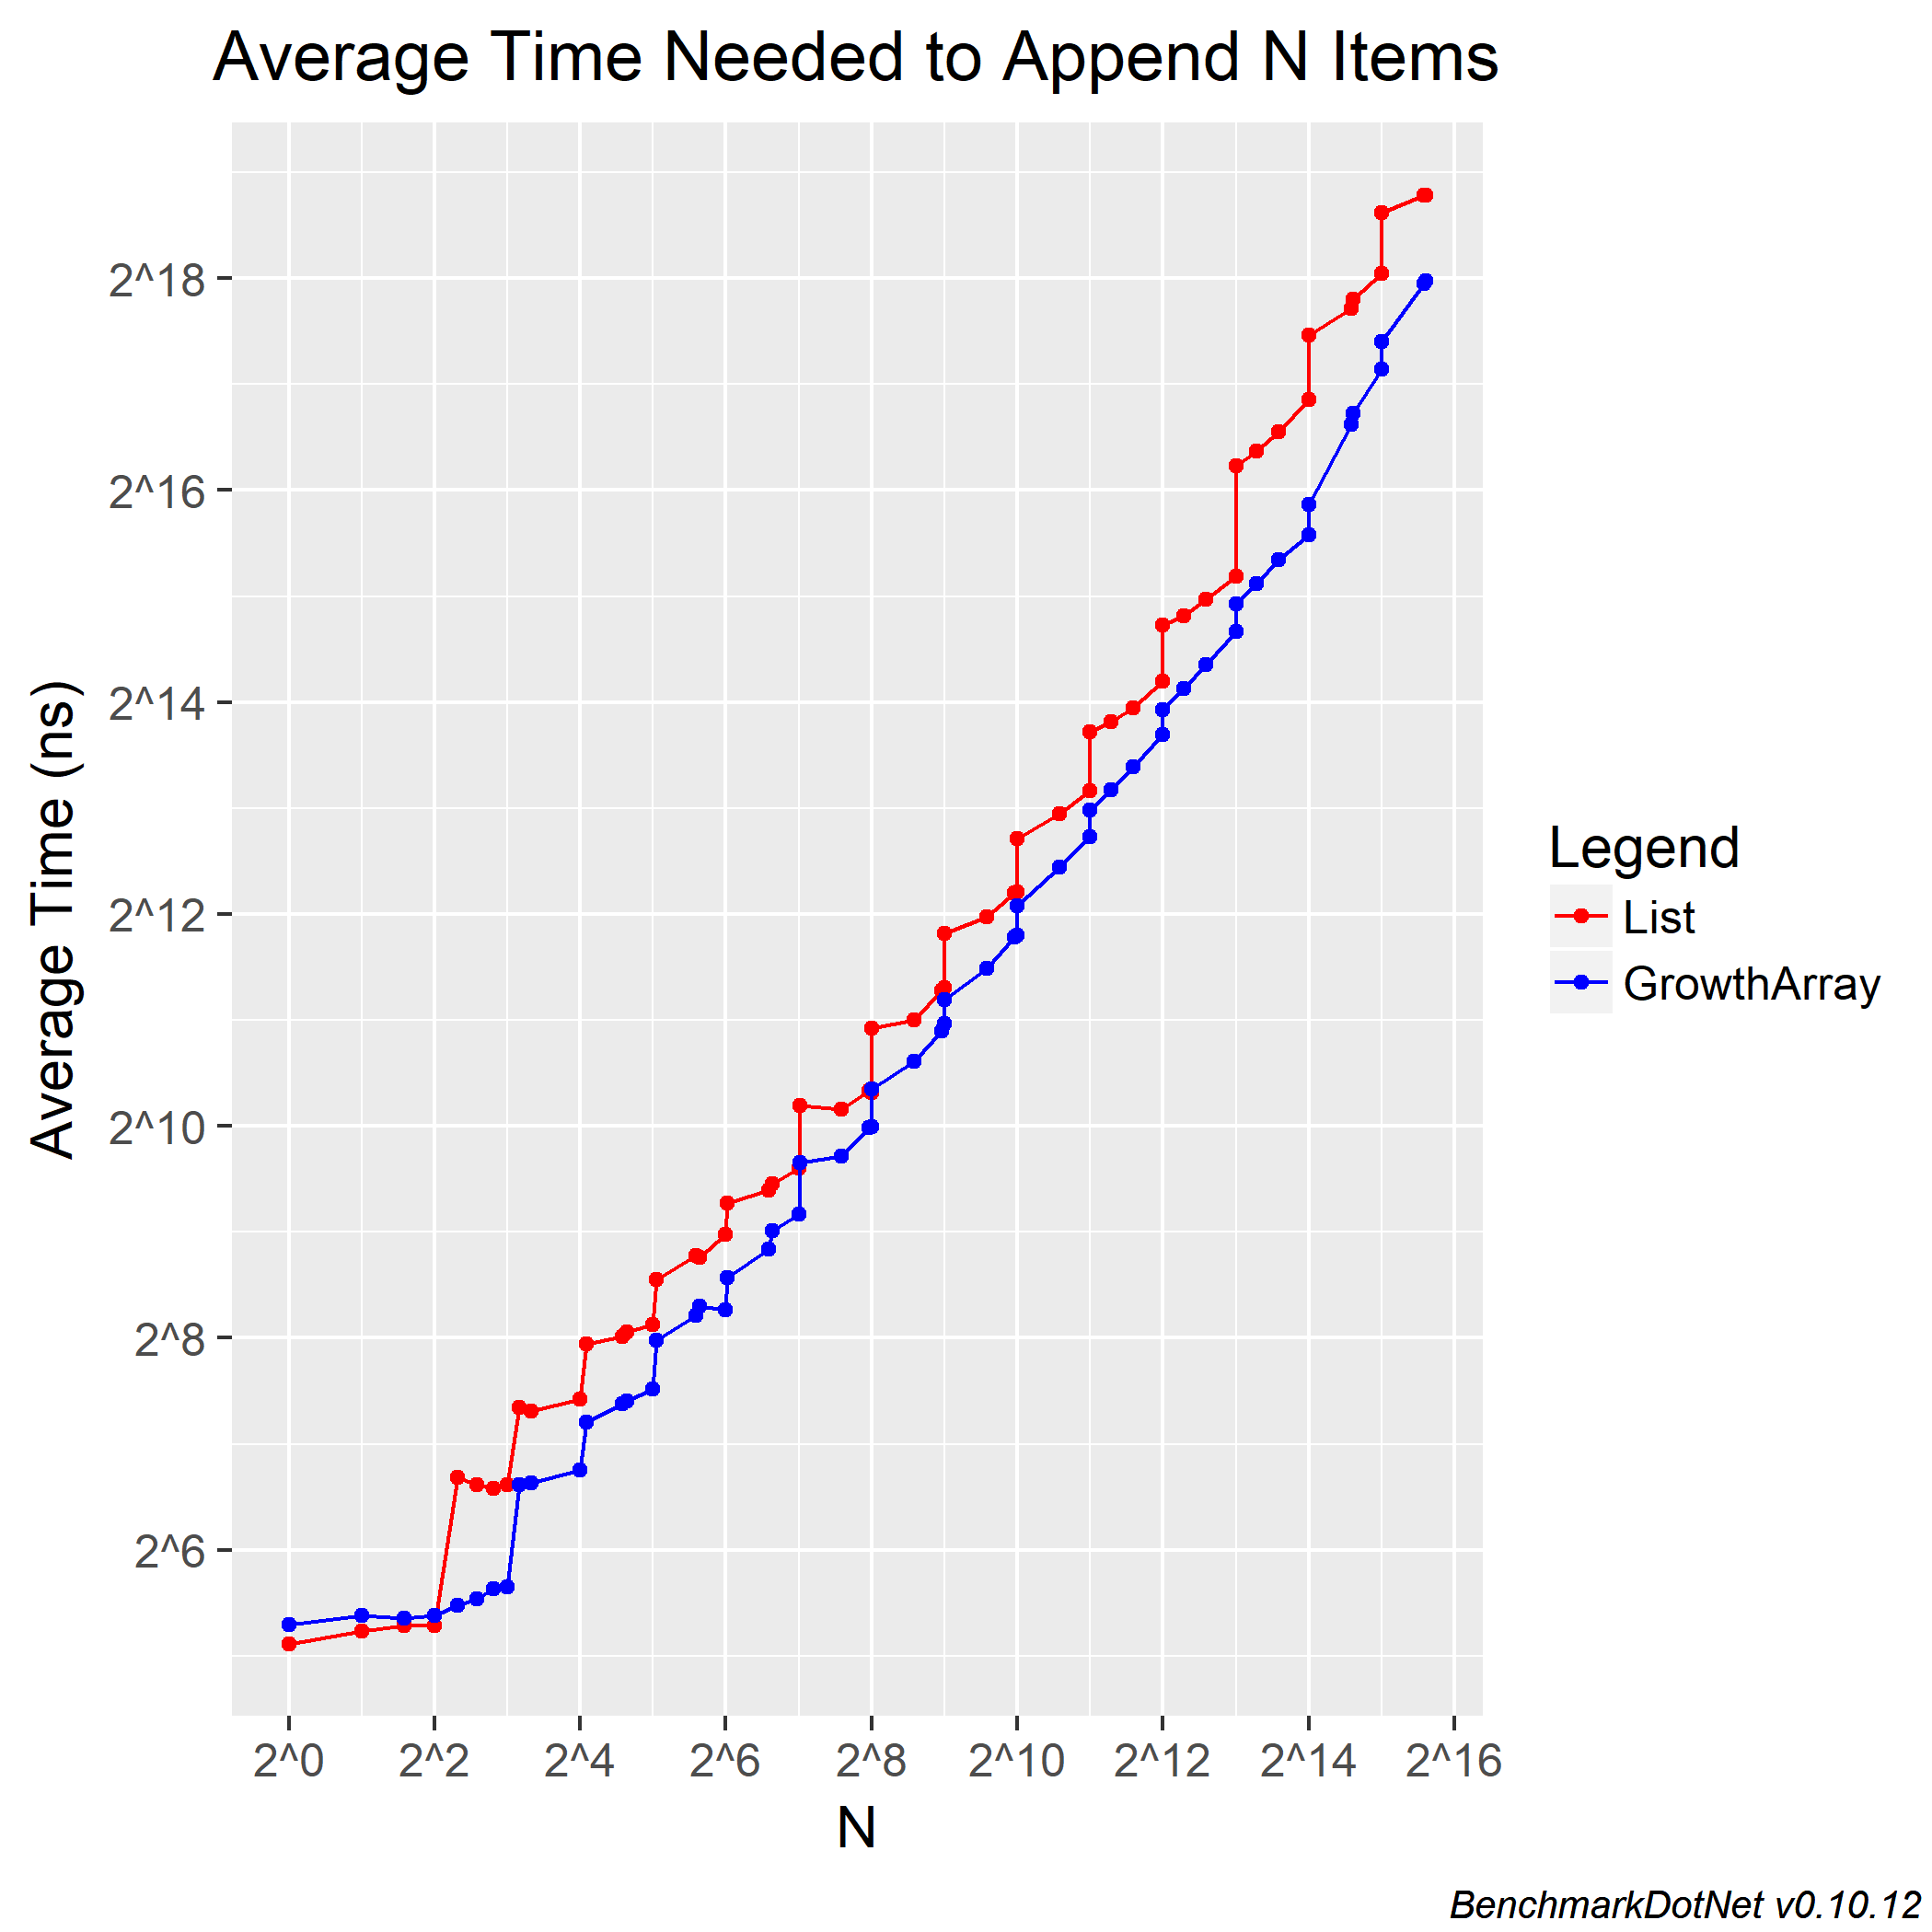
\includegraphics[width=3.25in]{Append-timeline}}
		\caption{Time measurements for appending}
	\end{minipage}\hfill
	\begin{minipage}{0.45\textwidth}
		\label{plot:2}
		\centering{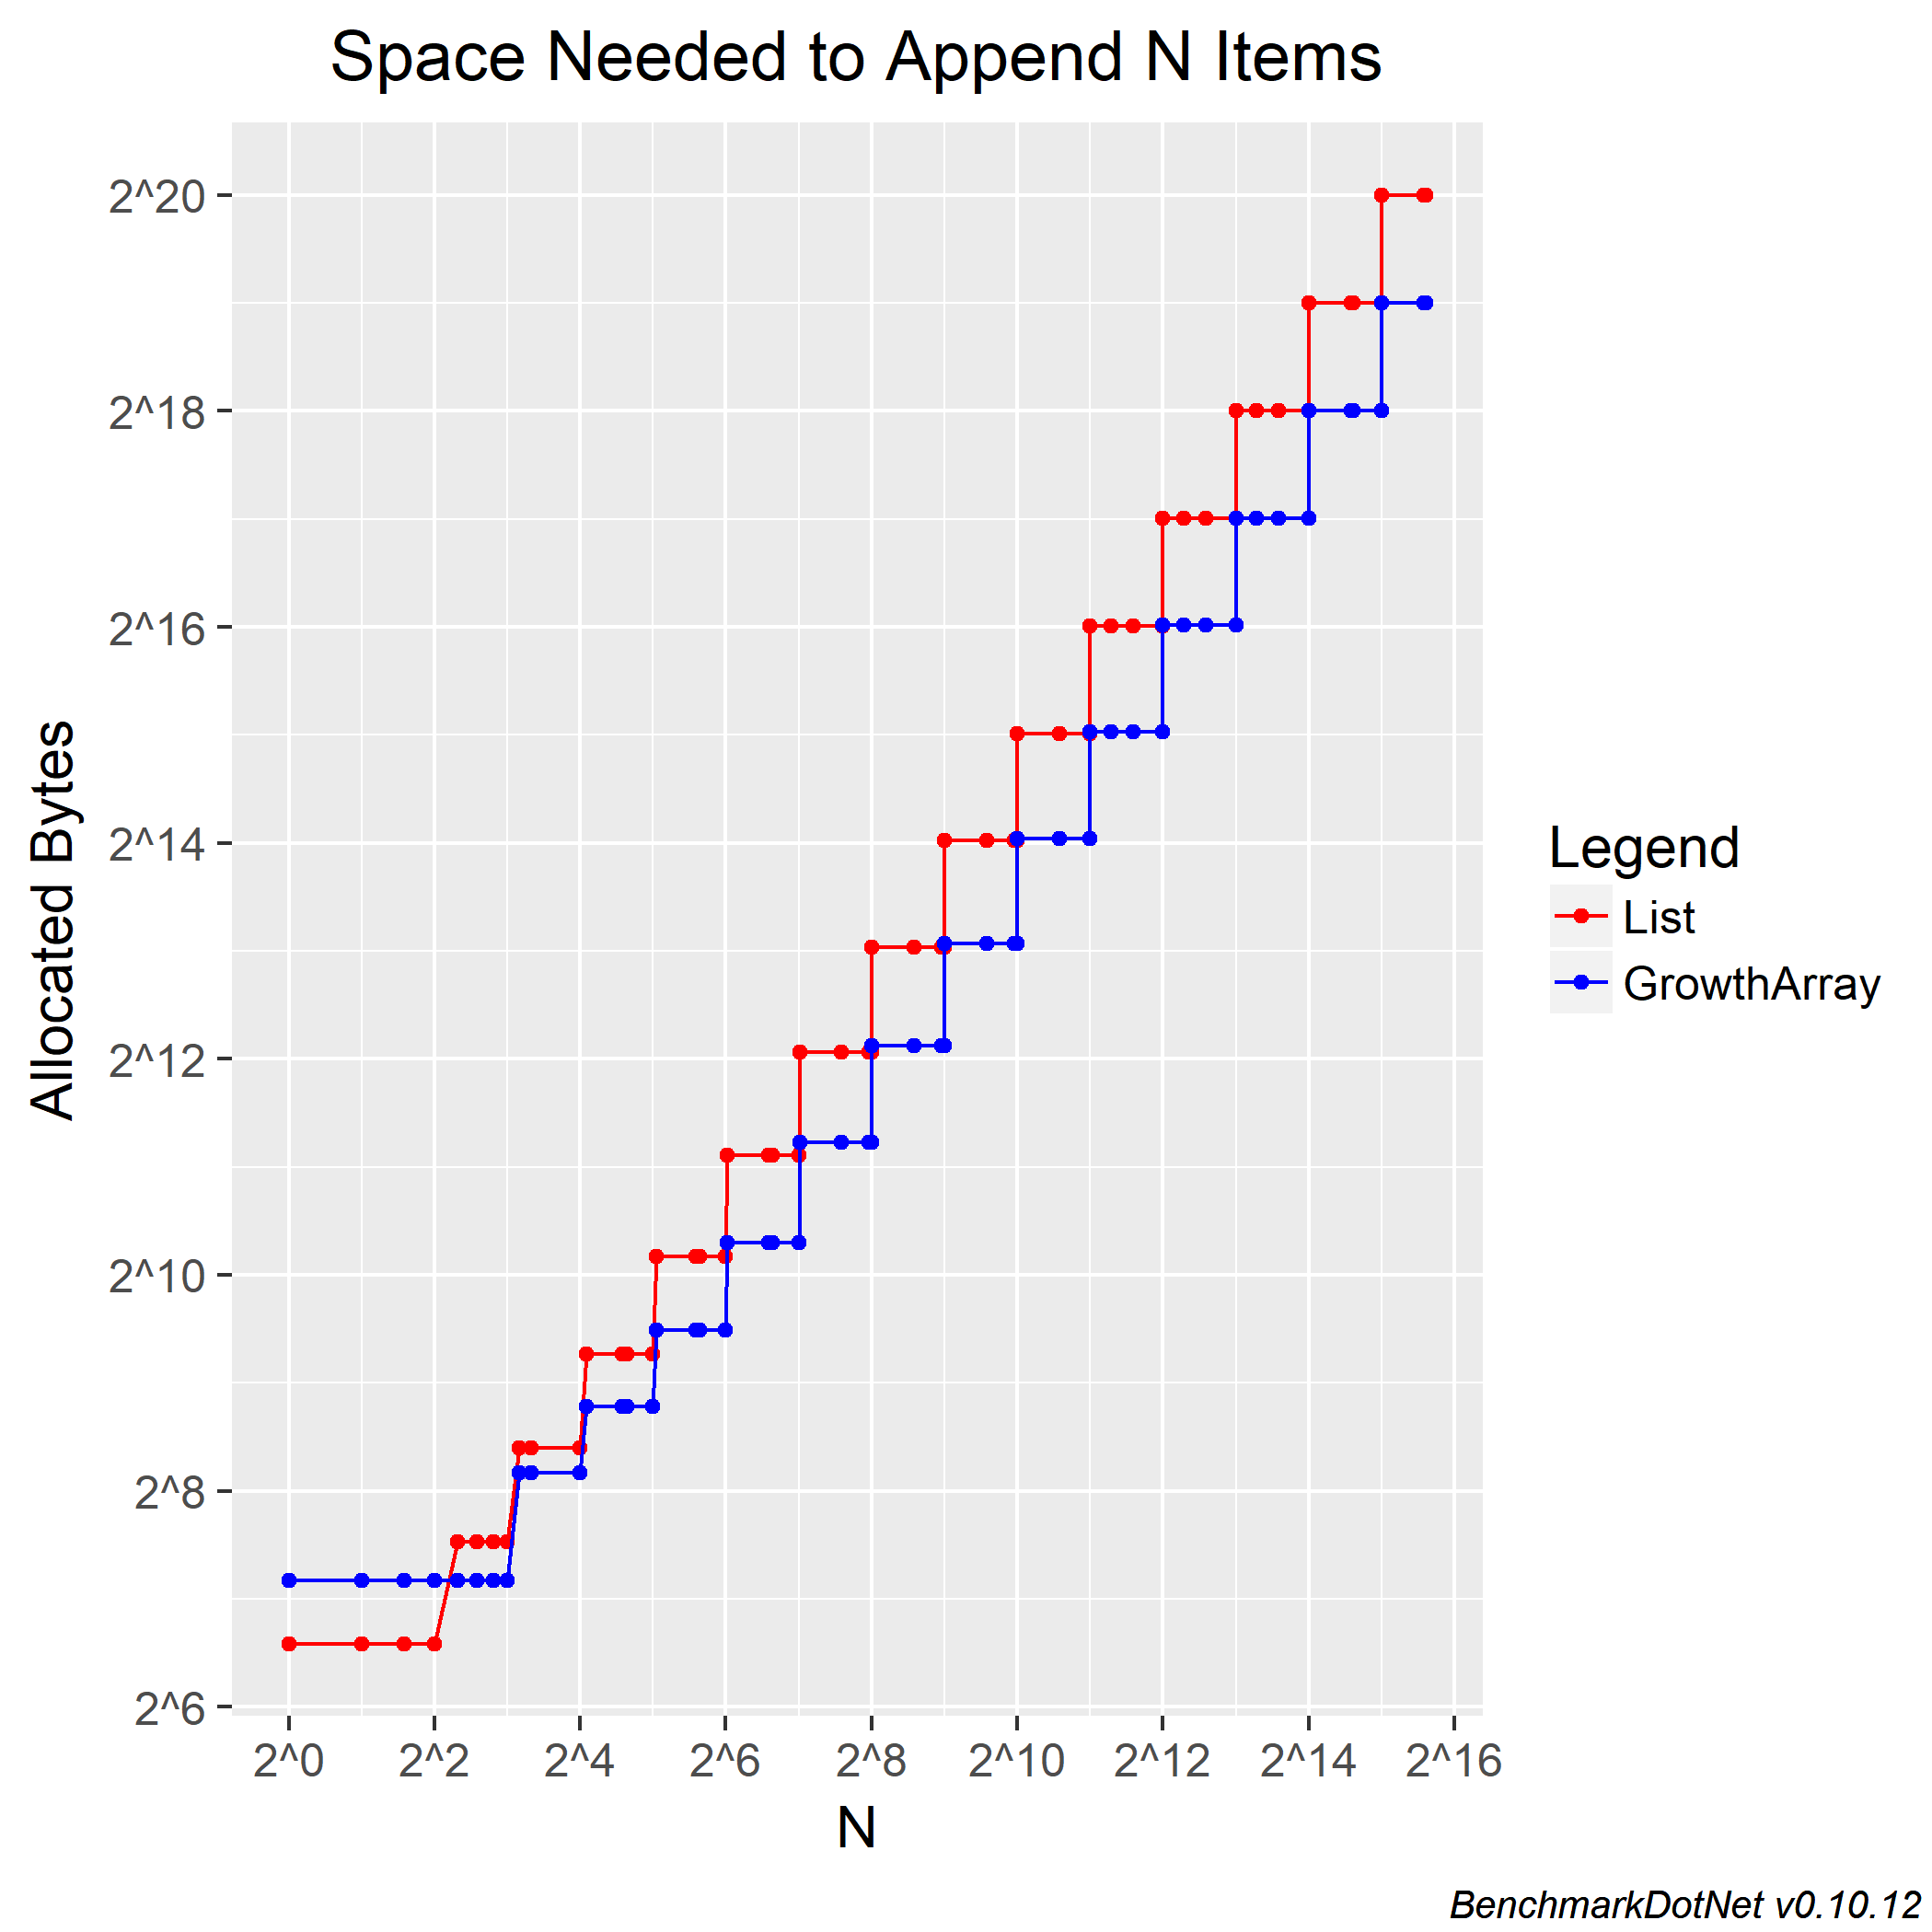
\includegraphics[width=3.25in]{Append-allocations}}
		\caption{Space measurements for appending}
	\end{minipage}
\end{figure}

\begin{figure}[H]
	\begin{minipage}{0.45\textwidth}
		\label{plot:3}
		\centering{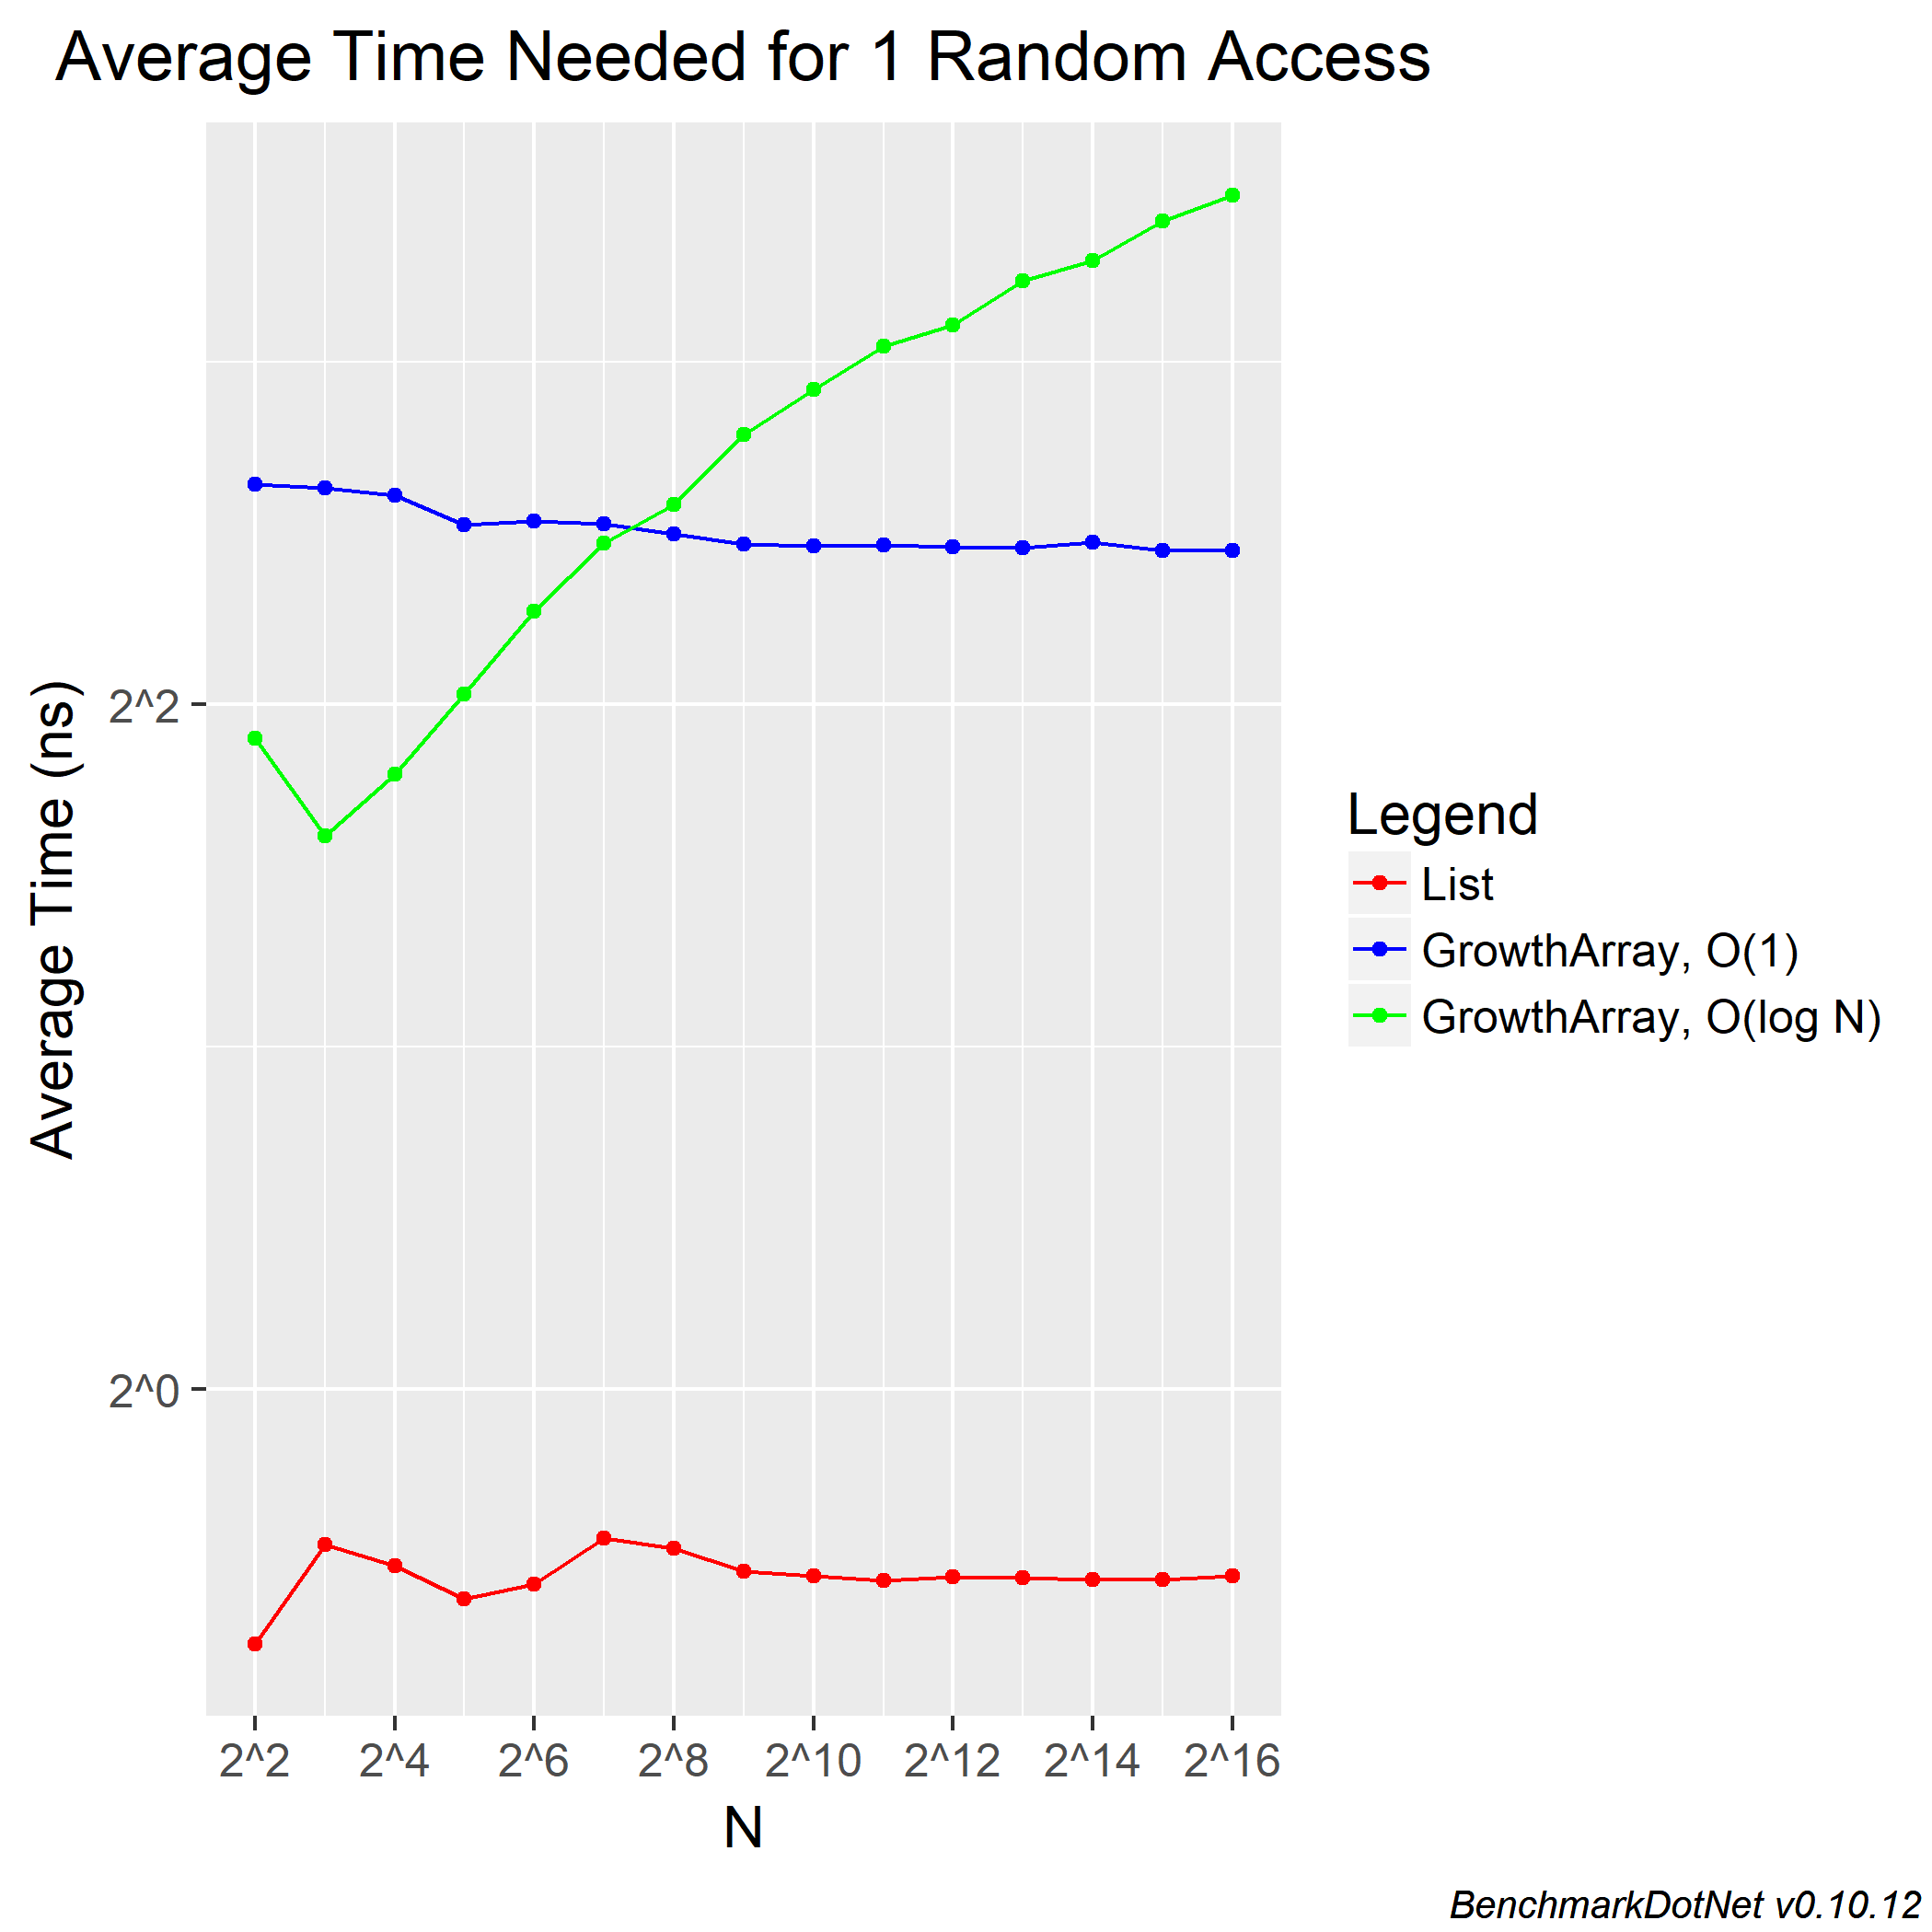
\includegraphics[width=3.25in]{GetItem-timeline}}
		\caption{Time measurements for indexing}
	\end{minipage}\hfill
	\begin{minipage}{0.45\textwidth}
		\label{plot:4}
		\centering{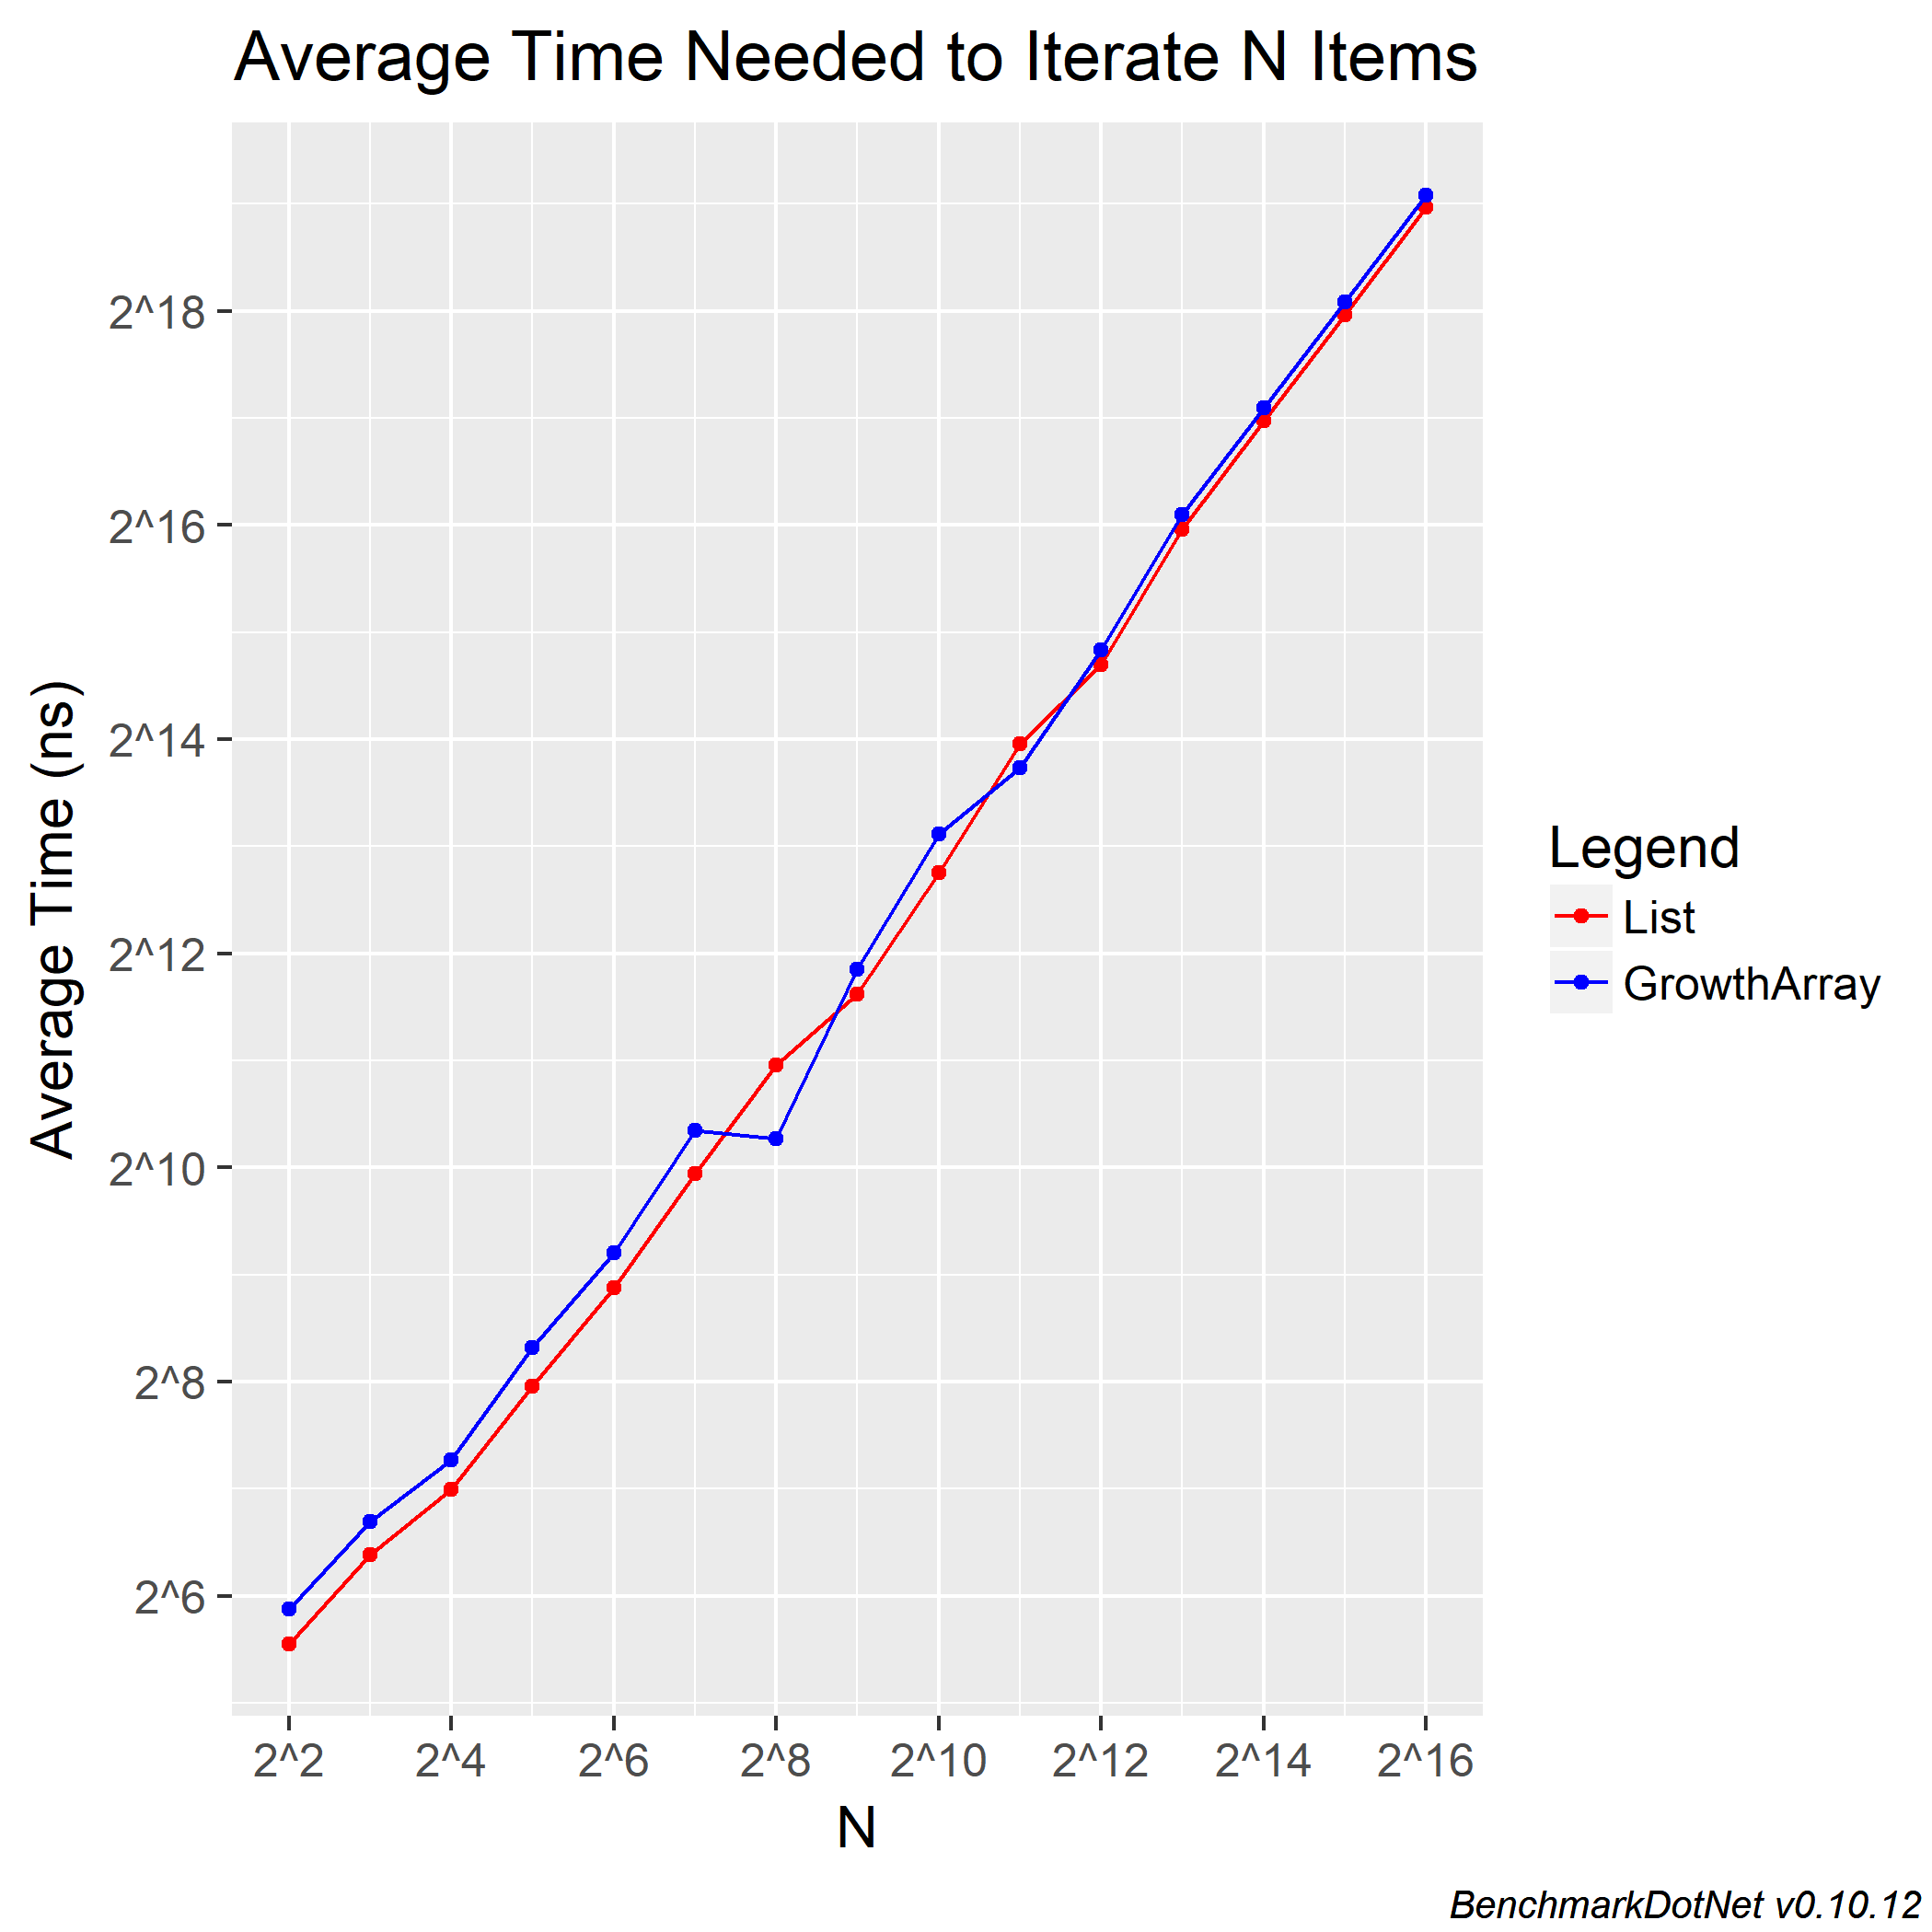
\includegraphics[width=3.25in]{Iteration-timeline}}
		\caption{Time measurements for iterating}
	\end{minipage}
\end{figure}

\begin{figure}[H]
	\begin{minipage}{\textwidth}
		\label{plot:5}
		\centering{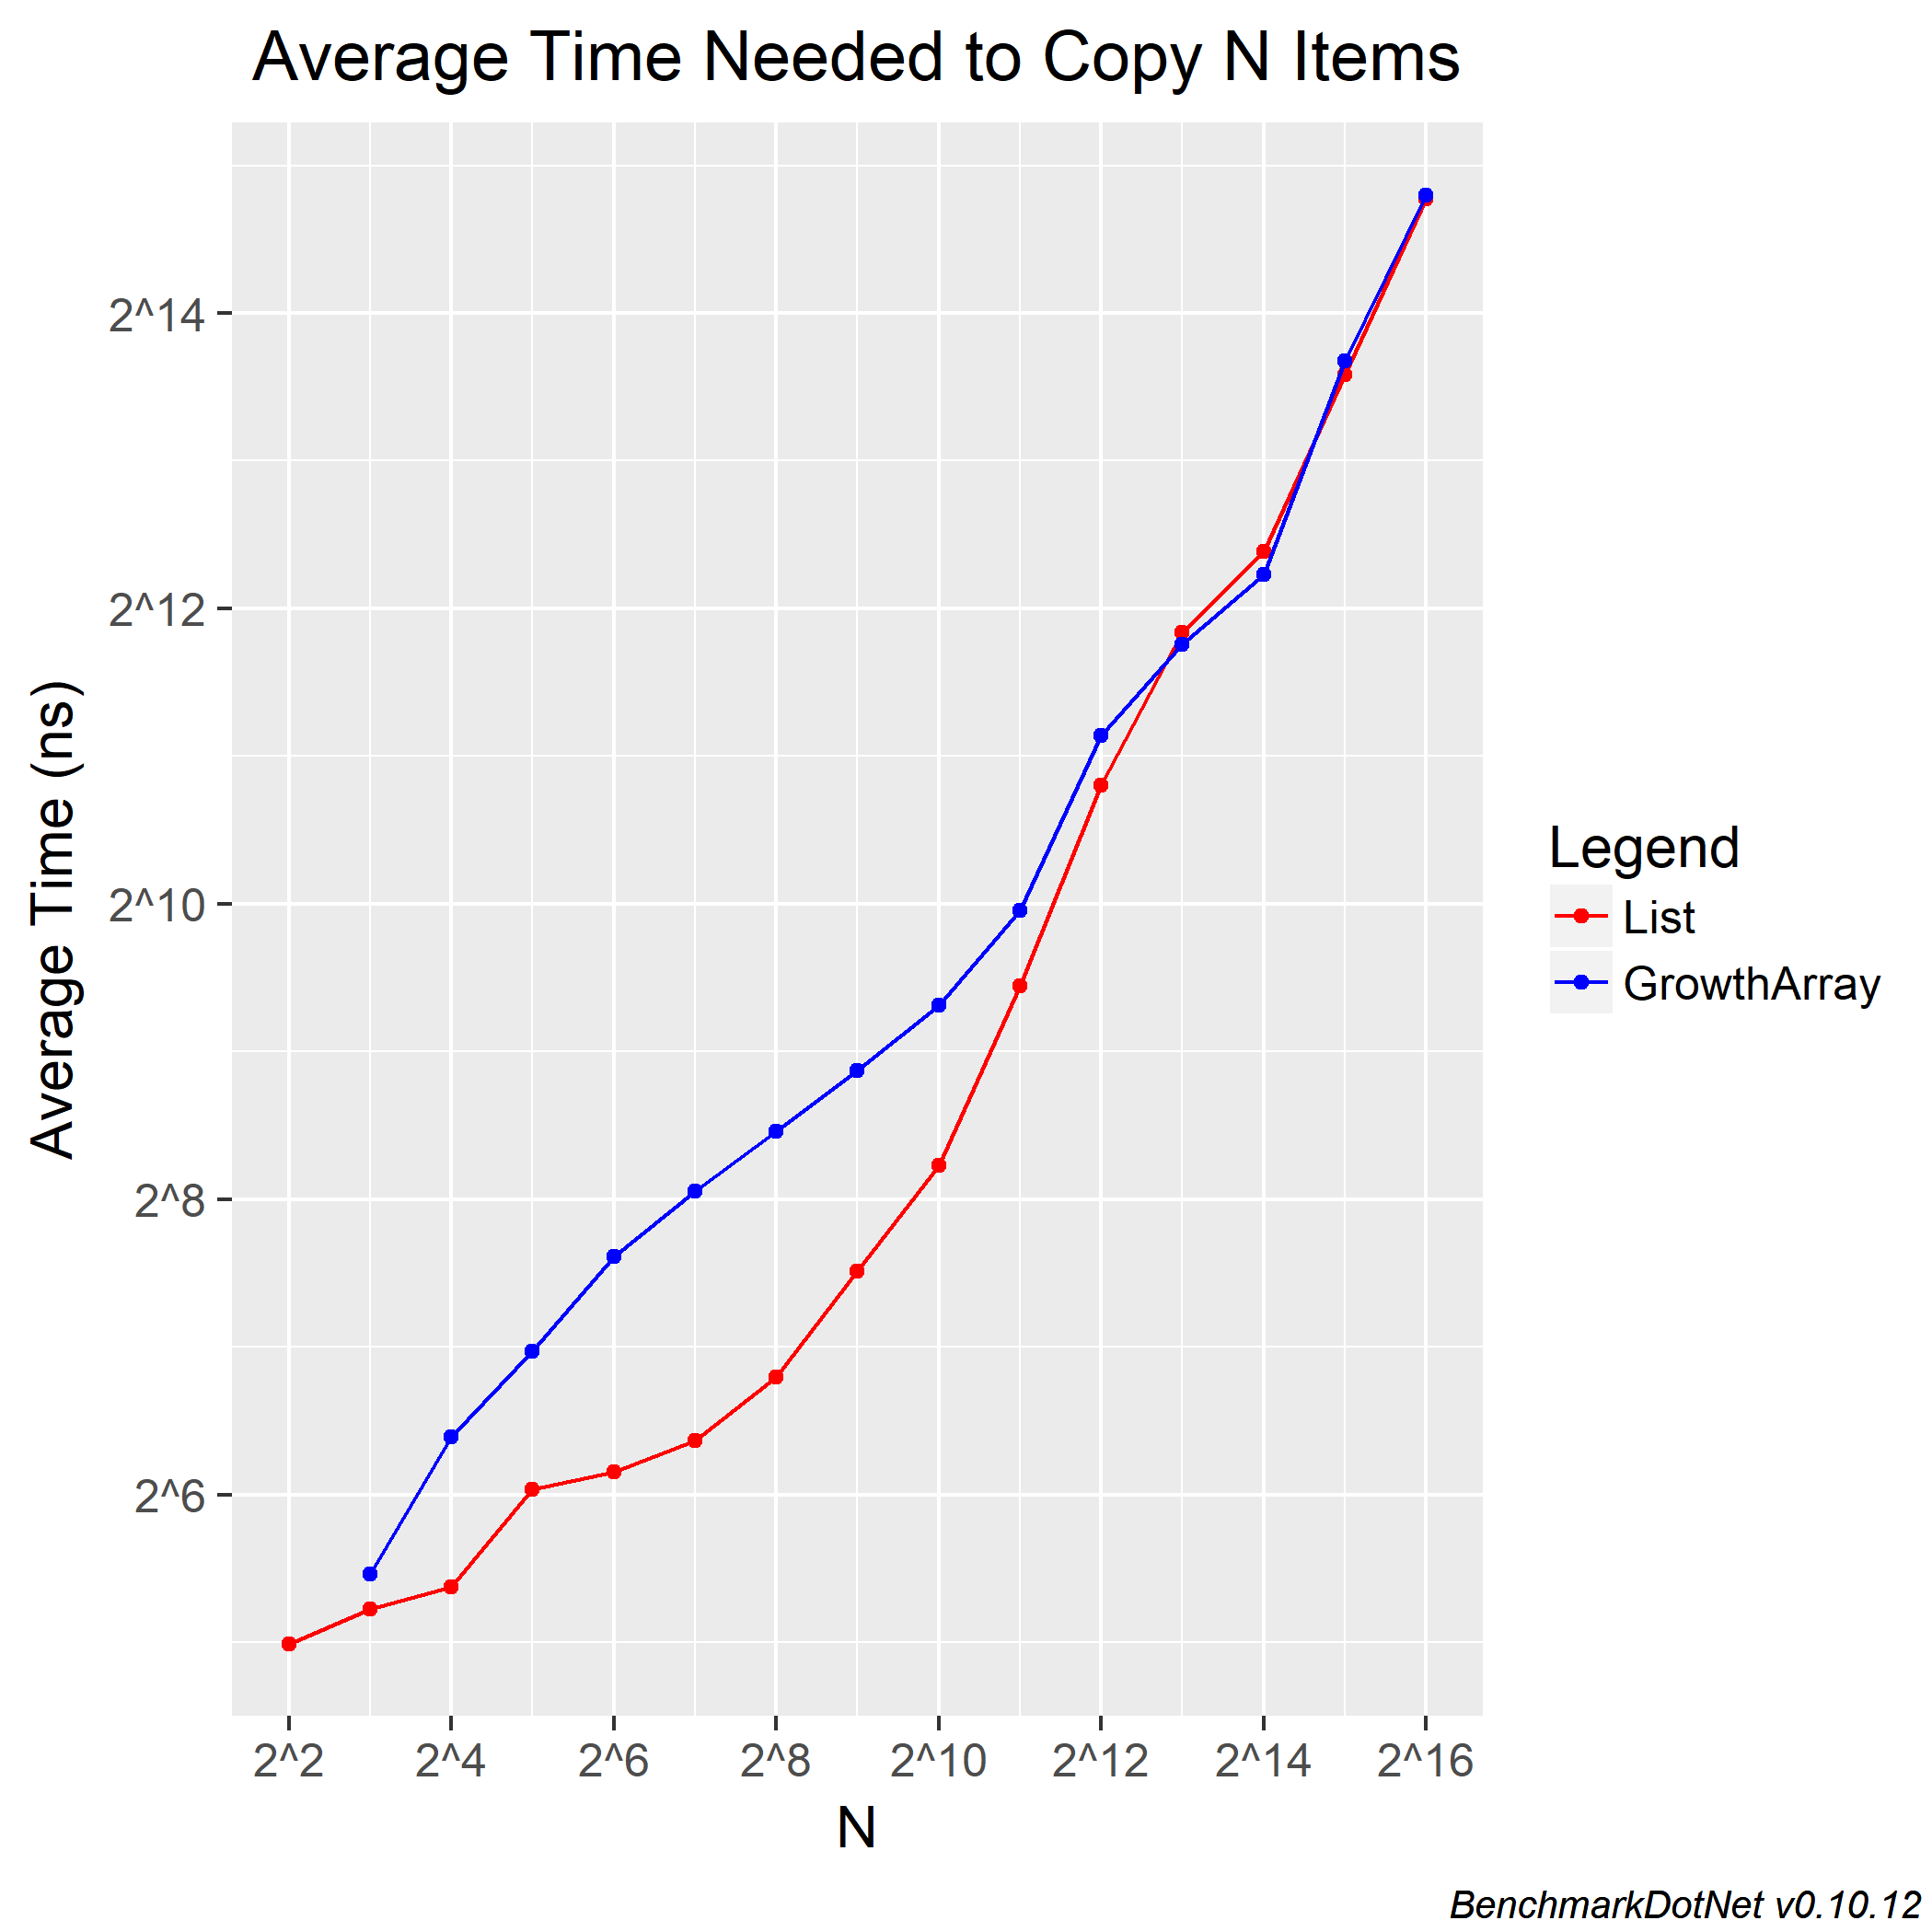
\includegraphics[width=3.25in]{Copying-timeline}}
		\caption{Time measurements for copying to raw arrays}
	\end{minipage}
\end{figure}

%% TODO: Why isn't \ref working?
Figures 4 and 5 show that growth arrays consistently outperform dynamic arrays at appending. Past $n = 4$, the blue line remains about one unit square below the red line for both graphs. Since the graphs are logarithmically scaled with one unit square representing a factor of $2$, I conclude that growth arrays use approximately half the time and half the space to append the same number of items as dynamic arrays for values of $n$ past $4$.

It misleadingly looks like the lines are touching for values of $n$ near powers of $2$. At these points, the blue and red lines appear to make vertical ``jumps.'' That is not what is really happening. The bottom end of each jump corresponds to when $n$ is a power of $2$, and the top end corresponds to when $n$ is one more than a power of $2$. The top end of each blue jump is close to the bottom end of each red jump, but it is incorrect to compare them since both points correspond to different values of $n$.

As you might guess, these jumps are where full capacity is reached and growth must occur. The sudden increase in time is mainly caused by the $O(n)$ memory allocation and (in dynamic arrays' case) the copying that happens when $\FuncGrow$ is called. Notice that the blue jumps are much less drastic than the red ones; this is because growth arrays do not make a copy of $n$ elements when they grow.

Figure 6 illustrates the graphs of 3 different random access algorithms, 2 of them for growth arrays. The constant time algorithms flat-line as they should, while the logarithmic time algorithm traces out a logarithmic curve. The dynamic array algorithm clearly beats both of the growth array algorithms: it appears to be approximately $8$ times faster than the constant time algorithm I introduced, and around $4$ times faster than the logarithmic time one at the point they are closest. An interesting observation is that the logarithmic time algorithm appears to outperform the blue constant time algorithm for values of $n$ that are $128$ or less.

Figures 7 and 8 show an interesting trend: the blue line converges towards the red line as $n$ gets very large. This supports the claim that I made in Sections \ref{subsec:Iterating} and \ref{subsec:ConvertRawArray} that not only do iteration and copying have the same time complexity for dynamic and growth arrays, their respective algorithms also have negligible time difference across data structures as $n$ gets very large. Also worth noting is the large gap that opens between the red and blue lines in Figure 8 for values of $n$ between $8$ and $4096$. This suggests that for small values of $n$, the extra overhead growth arrays introduce by iterating the tail's buffers is very significant.

For all benchmarks, BenchmarkDotNet consistently reported margins of error and standard deviation values on the order of $\frac{1}{100}$th of the measurement values.

	
	\section{Closing Remarks}
	
	In this paper, I developed the concept of growth arrays and showed that they are a viable replacement for dynamic arrays. I implemented several common dynamic array operations for growth arrays, and showed that for appending, growth arrays outperform dynamic ones both time- and memory-wise. I demonstrated that although growth arrays are slower at random access than dynamic arrays, it is still possible to index them in constant time. Finally, I showed that they perform comparably to dynamic arrays for iteration and conversion to raw arrays.

% Todo: Should have this paragraph?
Today, dynamic arrays are commonly used because they are reasonably efficient at appending. Since growth arrays are even faster at appending, it is possible that they could begin to supplant dynamic arrays if programming languages start adopting them in their standard libraries. It is also possible that the trade-offs growth arrays make to achieve faster appending could hinder their adoption, or have languages offer them as an alternative to dynamic arrays.

I will end this paper with the following open-ended questions, which may serve as inspiration for further research:

\begin{itemize}
	\item Can growth arrays' growth algorithm bring performance improvements to other array-based structures, such as circular queues or array-based stacks?
	\item Is there an efficient, constant time random access algorithm for growth arrays that works for all values of $\VarGrowthFactor$ and $\VarInitCapacity$?
	\item To what extent does growth arrays' fragmented structure result in performance losses due to poorer data locality? Can memory allocators offset these losses by allocating buffers close to each other?
	\item How can algorithms such as binary search and sorting be best implemented for growth arrays? Since growth arrays with $\VarGrowthFactor = 2$ have an evenly-divided structure, is there a better binary search algorithm for them?
\end{itemize}
	
	\newpage
	
	% Todo: Name 'Appendix', not 'Appendices'
\appendix
\appendixpage

\section{Proofs of $\sim$ Properties}

\subsection{$\sim$ is an Equivalence Relation}

\begin{proof}[Proof (Theorem \ref{thm:EquivalenceRelation})]
	Clearly, $\ExprNToInfty \dfrac{f}{f} = 1$, so $f \sim f$. Thus, $\sim$ is reflexive.
	
	Suppose $f \sim g$. Then $\ExprNToInfty \dfrac{f}{g} = 1$. Since both $\ExprNToInfty 1$ and $\ExprNToInfty \dfrac{f}{g}$ exist and the latter is nonzero, $\dfrac{\ExprNToInfty 1}{\ExprNToInfty (f / g)}$ = $\ExprNToInfty \dfrac{g}{f}$. Since the left-hand side evaluates to $1$, $g \sim f$. Thus, $\sim$ is symmetric.
	
	Suppose $f \sim g$ and $g \sim h$. By definition, $\ExprNToInfty \dfrac{f}{g} = 1$ and $\ExprNToInfty \dfrac{g}{h} = 1$. Since both limits exist, their product is $\ExprNToInfty \left( \dfrac{f}{g} \cdot \dfrac{g}{h} \right) = \ExprNToInfty \dfrac{f}{h}$. Since this product is $1$, $f \sim h$. Thus, $\sim$ is transitive.
\end{proof}

\subsection{$\sim$ Removes Lower-Order Terms}

\begin{proof}[Proof (Theorem \ref{thm:RemovesLowerOrderTerms})]
	Let $h = O(g)$. By definition, $h \leq cg$ for sufficiently large $n$, where $c$ is a positive constant. Dividing both sides by $f$ and taking the limit, $\ExprNToInfty \dfrac{h}{f} \leq \ExprNToInfty c \left( \dfrac{g}{f} \right)$. Since $\ExprNToInfty \dfrac{g}{f}$ exists and equals $0$, the right-hand side equals $c \cdot 0 = 0$. However, $\ExprNToInfty \dfrac{h}{f} \geq 0$ since both $h$ and $f$ are positive. By the squeeze theorem, $\ExprNToInfty \dfrac{h}{f} = 0$.
	
	Since $\ExprNToInfty \dfrac{f}{f}$ and $\ExprNToInfty \dfrac{h}{f}$ both exist,
	\begin{align*}
	\ExprNToInfty \dfrac{f + h}{f} = \ExprNToInfty \dfrac{f}{f} + \ExprNToInfty \dfrac{h}{f} = 1 + 0 = 1
	\end{align*}
	It follows that $f + h = f + O(g) \sim f$.
\end{proof}

\subsubsection{$f + c \sim f$ for Unbounded $f$}

\begin{proof}[Proof (Corollary \ref{coro:PlusConstant})]
	If $f$ is unbounded, $\ExprNToInfty \dfrac{c}{f} = 0$. Applying Theorem \ref{thm:RemovesLowerOrderTerms}, $f + c \sim f$.
\end{proof}

\subsection{$\sim$ Merges over $+$, $\times$, and $\div$}

\begin{proof}[Proof (Theorem \ref{thm:MergesOverOps})]
	% TODO: Prove statement for addition.
	
	The statement about multiplication is more easily proven. Since both $\ExprNToInfty \dfrac{f}{\Tweak{f}}$ and $\ExprNToInfty \dfrac{g}{\Tweak{g}}$ exist,
	\begin{align*}
	\ExprNToInfty \frac{fg}{\Tweak{f}\Tweak{g}} = \left( \ExprNToInfty \frac{f}{\Tweak{f}} \right) \left( \ExprNToInfty \frac{g}{\Tweak{g}} \right) = 1 \cdot 1 = 1
	\end{align*}
	It follows that $fg \sim \Tweak{f}\Tweak{g}$. If the limit for $g$ is flipped before multiplying, the following results:
	\begin{align*}
	\ExprNToInfty \frac{f / g}{\Tweak{f} / \Tweak{g}} = 1
	\end{align*}
	This shows that $\dfrac f g \sim \dfrac {\Tweak{f}} {\Tweak{g}}$.
\end{proof}

\subsubsection{$\sim$ Relations can be Algebraically Manipulated}

\begin{proof}[Proof (Corollary \ref{coro:BothSides})]
	Since $\sim$ is reflexive, $g \sim g$. Taking $\Tweak{g} = g$ for Theorem \ref{thm:MergesOverOps}, the corollary statement follows.
\end{proof}

\subsection{Asymptotic Functions Have the Same Big-O Class}

\begin{proof}[Proof (Theorem \ref{thm:SameBigOClass})]
	This will be a proof by contradiction. Assume $f = O(\Tweak{f})$ where $O(\Tweak{f}) \neq O(\Tweak{g})$. Then $\dfrac {O(\Tweak{f})} {O(\Tweak{g})} \neq 1$. However, $\ExprNToInfty \dfrac{f}{g} = \dfrac {O(\Tweak{f})} {O(\Tweak{g})}$, so $\ExprNToInfty \dfrac{f}{g} \neq 1$. It follows that $f \not\sim g$, which contradicts the given. Thus, it must be true that $f = O(\Tweak{g})$.
\end{proof}

\subsection{Asymptotic Functions may be Swapped in Strict Asymptotic Inequalities}

\begin{proof}[Proof (Theorem \ref{thm:InterchangeableInInequality})]
	By definition, $\ExprNToInfty \dfrac{f}{\Tweak{f}} = 1$ and $\ExprNToInfty \dfrac{\Tweak{f}}{\TweakSecond{f}} < 1$. Since both limits exist,
	\begin{align*}
	\ExprNToInfty \frac{f}{\TweakSecond{f}} = \left( \ExprNToInfty \frac{f}{\Tweak{f}} \right) \left( \ExprNToInfty \frac{\Tweak{f}}{\TweakSecond{f}} \right) < 1 \cdot 1 = 1
	\end{align*}
	It follows that $f \FluteLess \TweakSecond{f}$.
	
	The second statement may be proved in a similar manner. Since $\sim$ is symmetric, $\TweakSecond{g} \sim g$. Applying the same argument as before,
	\begin{align*}
	\ExprNToInfty \frac{\Tweak{g}}{g} = \left( \ExprNToInfty \frac{\Tweak{g}}{\TweakSecond{g}} \right) \left( \ExprNToInfty \frac{\TweakSecond{g}}{g} \right) < 1 \cdot 1 = 1
	\end{align*}
	Thus, $\Tweak{g} \FluteLess g$.
\end{proof}

\subsubsection{Asymptotic Functions may be Swapped in Non-Strict Asymptotic Inequalities}

\begin{proof}[Proof (Corollary \ref{coro:InterchangeableInNonStrictInequality})]
	Suppose $f \sim \Tweak{f}$ and $\Tweak{f} \FluteLeq \TweakSecond{f}$. By definition, $\Tweak{f} \FluteLess \TweakSecond{f}$ or $\Tweak{f} \sim \TweakSecond{f}$. In the first case, from Theorem \ref{thm:InterchangeableInInequality} $f \FluteLess \TweakSecond{f}$. In the second case, since $\sim$ is transitive $f \sim \TweakSecond{f}$. In both cases, it is true that $f \FluteLeq \TweakSecond{f}$.
	
	The second statement is, again, proved in a similar manner. If $\Tweak{g} \FluteLeq \TweakSecond{g}$, then $\Tweak{g} \FluteLess \TweakSecond{g}$ or $\Tweak{g} \sim \TweakSecond{g}$. In the first case, $\Tweak{g} \FluteLess g$; in the second, $\Tweak{g} \sim g$. In both cases, $\Tweak{g} \FluteLeq g$.
\end{proof}

\subsubsection{$\FluteLess$ and $\FluteLeq$ Relations can be Algebraically Manipulated}

\begin{proof}[Proof (Theorem \ref{thm:BothSidesInequality})]
	Suppose that $f \FluteLess g$. By definition, $\ExprNToInfty \dfrac{f}{g} < 1$. For any function $h$, $\ExprNToInfty \dfrac{fh}{gh} < 1$ and $\ExprNToInfty \dfrac{f / h}{g / h} < 1$, so respectively $fh \FluteLess gh$ and $\dfrac{f}{h} \FluteLess \dfrac{g}{h}$.
	
	If I suppose $f \FluteLeq g$, then $f \FluteLess g$ or $f \sim g$. The first statement implies $fh \FluteLess gh$, and the second implies $fh \sim gh$ (from Corollary \ref{coro:BothSides}). In either case, $fh \FluteLeq gh$. Using the same logic, it is true that $\dfrac{f}{h} \FluteLeq \dfrac{g}{h}$.
\end{proof}
	
	\newpage
	
	\begin{flushleft}
\begin{thebibliography}{9}

\bibitem{tildedef}
	de Bruijn, Nicolaas G. \textit{Asymptotic Methods in Analysis}. Dover Publications, 1981.

\bibitem{littleodef}
	Cormen et al. \textit{Introduction to Algorithms, Second Edition}. The MIT Press, 2001.

\bibitem{amortized}
	Fiebrink, Rebecca. \textit{Amortized Analysis Explained}. Princeton University, 2007. Available at \texttt{https://www.cs.princeton.edu/\textasciitilde{}fiebrink/423/AmortizedAnalysisExplained\_Fiebrink.pdf}.

\bibitem{fptables}
	Fog, Agner. \textit{Lists of instruction latencies, throughputs and micro-operation breakdowns for Intel, AMD and VIA CPUs}. Technical University of Denmark, 2017. Available at \texttt{http://www.agner.org/optimize/instruction\_tables.pdf}.

\bibitem{ceillog2}
	Leiserson et al. \textit{Using de Bruijn sequences to Index a 1 in a Computer Word}. MIT Laboratory for Computer Science, 1998. Available at \texttt{http://supertech.csail.mit.edu/papers/debruijn.pdf}.

\end{thebibliography}
\end{flushleft}

\end{document}
